\documentclass[12pt,letterpaper,final]{article}

%\documentstyle[12pt,graphicx,natbib,hyperref,Sweave,rotating]{article}

\usepackage{Sweave}
\usepackage{graphicx}
\usepackage{natbib}
\usepackage{hyperref}
\usepackage{caption}
\usepackage{rotating}
\usepackage{verbatim}
\usepackage{textcomp}

\setlength{\oddsidemargin}{0in}
\setlength{\textwidth}{6.15in}
\setlength{\topmargin}{0.5in}
\setlength{\textheight}{22cm}
\setlength{\headheight}{0in}
\setlength{\headsep}{0in}
\setlength{\parskip}{5pt plus 2pt minus 3pt}

\marginparwidth2cm
\marginparsep0.2cm
\marginparpush0.2cm
%\tabcolsep0pt

\def\thefootnote{\fnsymbol{footnote}}
\setcounter{footnote}{1}

\renewcommand{\baselinestretch}{1.2}
\renewcommand{\labelenumi}{(\roman{enumi})}

\renewcommand{\topfraction}{1.0}
\renewcommand{\bottomfraction}{1.0}
\renewcommand{\textfraction}{0.0}
\renewcommand{\floatpagefraction}{1.0}

\newtheorem{definition}{Definition}
\newtheorem{theorem}{Theorem}
\newtheorem{lemma}[theorem]{Lemma}
\newtheorem{claim}[theorem]{Claim}
\newtheorem{fact}[theorem]{Fact}

% to get nice proofs ...
\newcommand{\qedsymb}{\mbox{ }~\hfill~{\rule{2mm}{2mm}}}
\newenvironment{proof}{\begin{trivlist}
\item[\hspace{\labelsep}{\bf\noindent Proof: }]
}{\qedsymb\end{trivlist}}

\def\printindex{\input{\jobname.ind}}

\newfont{\msymb}{cmsy10 scaled 1000}

\def\nullset{\mbox{\O}}
\def\R{{I\!\!R}}
\def\N{{I\!\!N}}
\def\C{{C\!\!\!\!I}}

\def\convdist{\stackrel{d}{\longrightarrow}}
\def\convlaw{\stackrel{L}{\longrightarrow}}
\def\convweak{\stackrel{w}{\longrightarrow}}
\def\convprob{\stackrel{p}{\longrightarrow}}
\def\convmean#1{\stackrel{#1}{\longrightarrow}}
\def\convas{\stackrel{a.s.}{\longrightarrow}}
\def\convwp{\stackrel{w.p.1}{\longrightarrow}}

\def\A{\mbox{\msymb A}}
\def\B{\mbox{\msymb B}}
\def\H{\mbox{\msymb H}}
\def\P{\mbox{\msymb P}}
\def\S{\mbox{\msymb S}}
\def\X{\mbox{\msymb X}}
\def\Y{\mbox{\msymb Y}}

\def\u0{\underline{0}}
\def\ua{\underline{a}}
\def\ub{\underline{b}}
\def\ud{\underline{d}}
\def\ug{\underline{g}}
\def\ueta{\underline{\eta}}
\def\umu{\underline{\mu}}
\def\utheta{\underline{\theta}}
\def\uvartheta{\underline{\vartheta}}
\def\UT{\underline{T}}
\def\ut{\underline{t}}
\def\UU{\underline{U}}
\def\uu{\underline{u}}
\def\OX{\overline{X}}
\def\UX{\underline{X}}
\def\ux{\underline{x}}
\def\UY{\underline{Y}}
\def\uy{\underline{y}}
\def\UZ{\underline{Z}}
\def\uz{\underline{z}}

%\parskip 0.1in
\pagenumbering{arabic}    %  Start using 1,2,... as page numbers.
\pagestyle{plain}         %  Page numbers in middle bottom of page.
%\setcounter{page}{80}  % XXXXXXXXXXXXXXXXX
%\setcounter{theorem}{5} % XXXXXXXXXXXXXXXXX
%\setcounter{definition}{10} % XXXXXXXXXXXXXXXXX

\parindent 0in

\makeindex


\begin{document}

\Sconcordance{concordance:lect_main.tex:lect_main.Rnw:%
1 163 1}
\Sconcordance{concordance:lect_main.tex:./lect_acknow.Rnw:ofs 164:%
1 40 1}
\Sconcordance{concordance:lect_main.tex:lect_main.Rnw:ofs 205:%
166 10 1}
\Sconcordance{concordance:lect_main.tex:./lect_chapter5.Rnw:ofs 216:%
1 62 1 1 4 6 0 1 2 12 1 1 7 6 0 5 2 8 0 1 2 1 5 4 0 4 2 1 3 1 2 1 3 1 2 %
1 3 1 2 1 3 1 2 1 3 1 2 8 0 1 2 80 1 1 2 12 0 2 1 1 2 1 3 1 0 1 2 1 0 1 %
2 1 0 1 2 1 0 1 2 5 0 1 1 5 0 1 1 5 0 1 1 7 0 1 2 2 1 1 2 1 0 1 1 1 3 1 %
0 1 5 3 0 1 5 3 0 1 5 3 0 1 5 3 0 1 5 3 0 1 2 4 0 1 2 2 1 1 2 1 0 4 2 4 %
0 1 2 52 1 1 7 6 0 2 2 5 0 2 2 1 1 1 2 1 1 1 2 1 1 4 0 1 2 1 1 1 5 4 0 %
1 2 5 0 2 2 1 1 1 2 1 1 1 2 1 1 1 3 1 1 1 2 1 1 1 3 1 1 1 2 1 1 1 3 1 1 %
1 2 1 1 1 3 1 1 1 2 1 1 1 3 1 1 4 0 1 2 25 1 1 2 14 0 1 2 18 0 1 3 15 0 %
1 2 24 0 1 3 10 0 1 2 13 0 1 2 20 0 1 2 26 1 1 2 1 0 6 2 4 0 1 2 1 1 1 %
2 1 0 2 2 4 0 1 2 15 1 1 2 1 0 4 2 1 4 2 0 1 5 3 0 1 6 8 0 1 2 1 1 1 2 %
1 0 2 2 4 0 1 2 18 1 1 2 1 0 9 2 4 0 1 2 1 1 1 2 1 0 2 2 4 0 1 2 3 1 1 %
2 1 0 1 9 11 0 1 2 25 1 1 2 1 0 1 2 1 1 18 0 1 2 1 1 7 0 2 1 18 0 1 2 4 %
0 2 2 5 0 1 2 1 3 6 0 1 2 3 1 1 2 1 0 1 2 4 0 1 2 1 3 6 0 1 2 3 1 1 2 1 %
0 1 2 1 1 26 0 1 3 5 0 1 2 1 1 1 4 3 0 1 1 16 0 1 3 5 0 1 2 4 1 1 12 11 %
0 1 3 1 0 1 1 4 0 1 2 13 1 1 2 1 0 1 2 1 1 11 0 1 5 7 0 2 2 7 0 1 7 9 0 %
1 2 39 1 1 2 1 0 1 2 3 1 2 2 1 0 2 2 1 0 2 2 1 0 2 2 5 0 1 2 1 1 1 2 1 %
0 1 2 5 1 4 0 1 2 2 1 1 2 1 0 1 2 2 1 1 3 1 0 2 1 4 0 1 2 9 1 1 2 1 0 1 %
1 1 6 4 0 1 6 4 0 1 7 5 0 1 7 5 0 1 9 7 0 1 9 7 0 1 2 4 0 1 2 22 1 1 3 %
2 0 2 2 2 1 1 2 2 1 1 2 2 1 1 2 2 1 1 2 2 1 1 2 2 1 4 0 1 2 14 1 1 2 1 %
0 1 1 1 2 1 3 2 0 2 3 2 0 1 2 4 0 1 2 6 1 1 2 1 0 2 2 2 1 1 2 2 1 1 2 2 %
1 1 2 2 1 1 5 3 0 1 1 1 3 1 0 1 1 4 0 1 2 5 1 1 2 1 0 4 2 4 0 1 2 37 1 %
1 2 1 0 3 2 2 1 1 2 2 1 1 2 2 1 1 2 2 1 4 0 1 2 1 1 1 3 2 0 1 2 2 1 1 7 %
8 0 1 2 5 1 1 2 5 0 1 2 71 1 1 2 1 0 3 2 1 7 5 0 1 2 7 0 1 2 1 1 1 2 1 %
0 3 2 1 7 5 0 1 2 7 0 1 2 10 1 1 4 3 0 1 1 4 0 1 2 1 1 1 2 1 0 1 1 4 0 %
1 2 40 1}
\Sconcordance{concordance:lect_main.tex:lect_main.Rnw:ofs 1762:%
178 31 1}



\bibliographystyle{agsm}

\begin{titlepage}
\vspace*{4.5cm}
\begin{center}
{\LARGE \bf Stat 5810, Section 003} \\[0.5cm]
{\LARGE \bf Statistical Visualization I} \\[0.5cm]
{\LARGE \bf Fall 2018} \\[0.5cm]
~ \\[2cm]
{\bf Dr. J\"urgen Symanzik} \\[0.3cm]
Utah State University \\[0.3cm]
Department of Mathematics and Statistics \\[0.3cm]
3900 Old Main Hill \\[0.3cm]
Logan, UT 84322--3900 \\[0.8cm]
Tel.: (435) 797--0696 \\[0.3cm]
FAX: (435) 797--1822 \\[0.3cm]
e-mail: \verb|symanzik@math.usu.edu| \\[0.3cm]
Web: \url{http://www.math.usu.edu/~symanzik/}
\end{center}

\thispagestyle{empty}
\vfill
\end{titlepage}

\newpage

\thispagestyle{empty}

\vspace*{5cm}

%\begin{figure}[ht]
%\centering{\includegraphics[width=0.99\textwidth]{Scans//PhdcomicsCom_Plotting.jpg}}
%\caption{\label{PhdcomicsCom_Plotting}
%\url{http://www.phdcomics.com/comics/archive.php?comicid=1541}, \\
%Cartoon.
%}
%\end{figure}


\newpage


\setcounter{page}{1}

\tableofcontents

\newpage

%~
%
%\newpage

% !Rnw root = lect_main.Rnw

\section*{Acknowledgements}

This course uses some of the course materials provided by
Dr.\ Mike Minnotte (formerly USU, now with the University of
North Dakota) as held in the Fall 2006 semester. Additional materials
have been taken from other Statistical Graphics courses, such as the
ones offered by Dr.\ Di Cook (formerly Iowa State University; now Monash University:
\url{http://dicook.org/}) and
Dr.\ Dan Carr (George Mason University: \url{http://mason.gmu.edu/~dcarr/}).
Other examples and R code originate from 
Heike Hofmann, Paul Murrell, Carson Sievert,
Martin Theus, Antony Unwin, Simon Urbanek, 
Hadley Wickham, Lee Wilkinson, and others.
We are likely to include parts from additional authors and sources
that will be specified later during the semester.

Thanks are also due to 60+ students and guests who took 
the former ``Stat 6560: Graphical Methods'' and
the current ``Statistical Visualization I \& II'' courses
with me since the Spring 2009 semester 
for their valuable comments that helped
to improve, correct, and extend these lecture notes.

~\\
J\"urgen Symanzik, September 10, 2018.


%\begin{figure}[ht]
%\centering{\includegraphics[width=3.5in]{Scans//Zelazny_px_Fig.jpg}}
%\caption{\label{Zelazny_px_Fig}
%\cite{Ze2001}, p.~x, Cartoon.
%}
%\end{figure}

\newpage

%~\\
%
%\newpage
\addcontentsline{toc}{section}{Acknowledgements}

\newpage


\setcounter{page}{1}

%\SweaveInput{lect_chapter0.Rnw}
%\SweaveInput{lect_chapter0_Unwin_IntroRgda-knitr_mod.Rnw}
%\SweaveInput{lect_chapter11.Rnw}
% !Rnw root = lect_main.Rnw

\def\jsprivatechfour{1} % show additional details
%\def\jsprivatechfour{0} % do NOT show additional details


\section{Categorical Plots}

%{\bf (Based on \cite{Wa97}, Chapter 1 \& \cite{Tu83}, Chapter 2)}


\subsection{Which Plot Type to Choose?}\label{WhichPlotTypeToChoose}


Often, there exist many valid options how to display (categorical) data.

\cite{Ze2001}, p.~12, suggests the following project:
\begin{quotation}
``Sketch as many charts as you can think of using these data:
the more the better.''
\end{quotation}

\begin{center}
{\bf Percentage of January Sales by Region} \\[0.2cm]
\begin{tabular}{lcc}
 & ~~\underline{Co. A}~~ & ~~\underline{Co. B}~~ \\
North & 13\% & 39\% \\
South & 35\% &  6\% \\
East  & 27\% & 27\% \\
West  & 25\% & 28\% \\
\end{tabular}
\end{center}



\newpage


\centerline{\Large \bf Worksheet}~\\

\centerline{\hfill {\large \bf Your Name:} \underline{\hspace*{5cm}}}

~\\[1cm]

\fbox{\rule[-0.2in]{0in}{2in}\hspace*{3in}} ~~ \fbox{\rule[-0.2in]{0in}{2in}\hspace*{3in}} \\

\fbox{\rule[-0.2in]{0in}{2in}\hspace*{3in}} ~~ \fbox{\rule[-0.2in]{0in}{2in}\hspace*{3in}} \\

\fbox{\rule[-0.2in]{0in}{2in}\hspace*{3in}} ~~ \fbox{\rule[-0.2in]{0in}{2in}\hspace*{3in}} \\

%\framebox[3in]{\vspace*{2in}} ~~ \framebox[3in]{\vspace*{2in}} \\

%\framebox[3in]{\vspace*{2in}} ~~ \framebox[3in]{\vspace*{2in}} \\

%\framebox[3in]{\vspace*{2in}} ~~ \framebox[3in]{\vspace*{2in}} \\


\newpage


\if\jsprivatechfour 1

\centerline{\Large \bf Worksheet Answers}~\\

%\begin{figure}[ht]
%\centering{\includegraphics[width=5.0in]{Scans//Zelazny_p14_Fig.jpg}}
%\caption{\label{Zelazny_p14_Fig}
%\cite{Ze2001}, p.~14, Figure.
%}
%\end{figure}


\newpage


%\begin{figure}[ht]
%\centering{\includegraphics[width=4.0in]{Scans//Zelazny_p15_Text.jpg}}
%\caption{\label{Zelazny_p15_Text}
%\cite{Ze2001}, p.~15, Text.
%}
%\end{figure}


\newpage


%\begin{figure}[ht]
%\centering{\includegraphics[width=5.0in]{Scans//Zelazny_InClass1_2017_10_19.jpg}} \\[0.5cm]
%\centering{\includegraphics[width=5.0in]{Scans//Zelazny_InClass2_2017_10_19.jpg}}
%\caption{\label{Zelazny_InClass_2017_10_19}
%Graphs constructed in class on 10/19/2017.
%}
%\end{figure}


\newpage


%\begin{figure}[ht]
%\centering{\includegraphics[width=5.0in]{Scans//Zelazny_InClass1_2018_10_02.jpg}} \\[0.5cm]
%\centering{\includegraphics[width=5.0in]{Scans//Zelazny_InClass2_2018_10_02.jpg}}
%\caption{\label{Zelazny_InClass_2017_10_19}
%Graphs constructed in class on 10/2/2018.
%}
%\end{figure}


\else
{\bf Additional details will be provided after class.}
\fi


\newpage


\subsection{Categorical Plots in R}


Recall Section 2.4, {\it ``Sex Bias in Graduate Admissions''},
from \cite{FPP2007}, pp.~17--20, many of us are using in our introductory
Stat 1040 class.

These data represent
aggregate data on applicants to graduate school at Berkeley for the six largest 
departments in 1973, classified by admission and sex. 
These data are often used to discuss the issue whether the data show evidence of sex bias 
in admission practices. There were 2691 male applicants, of whom 1198 (44.5\%) 
were admitted, compared with 1835 female applicants of whom 557 (30.4\%) were admitted. 
Ultimately, this data set is frequently used for illustrating Simpson's paradox and does
not show any sex bias when properly analyzed. 
An effective graphical way to explain Simpson's Paradox is the BK--Plot,
summarized in \cite{Wa2002}.

In R, the data are stored in a a 3--dimensional array 
resulting from cross--tabulating 4526 observations on 3 variables. 
The variables and their levels are as follows: \\
\begin{center}
\begin{tabular}{l|l|l}
~~No~~ & ~~Name~~ & ~~Levels~~ \\
\hline   
1 & Admit & Admitted, Rejected \\
2 & Gender & Male, Female \\
3 & Dept & A, B, C, D, E, F \\
\end{tabular}
\end{center} ~\\


In R, this data set is accessible via:
\begin{Schunk}
\begin{Sinput}
> UCBAdmissions
\end{Sinput}
\begin{Soutput}
, , Dept = A

          Gender
Admit      Male Female
  Admitted  512     89
  Rejected  313     19

, , Dept = B

          Gender
Admit      Male Female
  Admitted  353     17
  Rejected  207      8

, , Dept = C

          Gender
Admit      Male Female
  Admitted  120    202
  Rejected  205    391

, , Dept = D

          Gender
Admit      Male Female
  Admitted  138    131
  Rejected  279    244

, , Dept = E

          Gender
Admit      Male Female
  Admitted   53     94
  Rejected  138    299

, , Dept = F

          Gender
Admit      Male Female
  Admitted   22     24
  Rejected  351    317
\end{Soutput}
\end{Schunk}

A better tabular representation can be obtained via:
\begin{Schunk}
\begin{Sinput}
> ftable(UCBAdmissions)
\end{Sinput}
\begin{Soutput}
                Dept   A   B   C   D   E   F
Admit    Gender                             
Admitted Male        512 353 120 138  53  22
         Female       89  17 202 131  94  24
Rejected Male        313 207 205 279 138 351
         Female       19   8 391 244 299 317
\end{Soutput}
\end{Schunk}

To obtain the totals as represented in \cite{FPP2007}, p.~18,
we have to sum over dimensions 2 and 3 in this 3--dimensional array:
\begin{Schunk}
\begin{Sinput}
> apply(UCBAdmissions, c(2, 3), sum)
\end{Sinput}
\begin{Soutput}
        Dept
Gender     A   B   C   D   E   F
  Male   825 560 325 417 191 373
  Female 108  25 593 375 393 341
\end{Soutput}
\begin{Sinput}
> #
> # also, margin.table prodoces the same result
> #
> margin.table(UCBAdmissions, 2:3)
\end{Sinput}
\begin{Soutput}
        Dept
Gender     A   B   C   D   E   F
  Male   825 560 325 417 191 373
  Female 108  25 593 375 393 341
\end{Soutput}
\end{Schunk}

To better understand over which dimensions we sum,
replace the \verb|c(2, 3)| option with possible
other indices, e.g., \verb|1| or \verb|c(1, 2)|.
Try a few more. \\
 

\newpage


\underline{Question:} \\
How can we calculate in R the percent admitted, as shown in 
\cite{FPP2007}, p.~18, Table~2? This can be done via
a single command line and does not require any loop!
And, which single digit do we have to change in our
previous R command to obtain the percent rejected?

%\begin{figure}[h]
%\centering{\includegraphics[width=4.0in]{Scans//FPP_p18_Table2.jpg}}
%\caption{\label{FPP_p18_Table2}
%\cite{FPP2007}, p.~18, Table~2.
%}
%\end{figure}


\underline{Answer:} \\
\if\jsprivatechfour 1
\begin{Schunk}
\begin{Sinput}
> # Percent admitted
> UCBAdmissions[1, , ] / apply(UCBAdmissions, c(2, 3), sum) * 100
\end{Sinput}
\begin{Soutput}
        Dept
Gender           A         B         C         D         E         F
  Male   62.060606 63.035714 36.923077 33.093525 27.748691  5.898123
  Female 82.407407 68.000000 34.064081 34.933333 23.918575  7.038123
\end{Soutput}
\begin{Sinput}
> # Percent rejected
> UCBAdmissions[2, , ] / apply(UCBAdmissions, c(2, 3), sum) * 100
\end{Sinput}
\begin{Soutput}
        Dept
Gender          A        B        C        D        E        F
  Male   37.93939 36.96429 63.07692 66.90647 72.25131 94.10188
  Female 17.59259 32.00000 65.93592 65.06667 76.08142 92.96188
\end{Soutput}
\end{Schunk}
\else
{\bf Additional details will be provided after class.}
\fi


\newpage


\subsubsection{Pie Charts}


Let us concentrate on the popularity of the six majors first,
i.e., the total number of admissions for each of these majors.

In R, these application numbers can be calculated via:
\begin{Schunk}
\begin{Sinput}
> apply(UCBAdmissions, 3, sum)
\end{Sinput}
\begin{Soutput}
  A   B   C   D   E   F 
933 585 918 792 584 714 
\end{Soutput}
\end{Schunk}

Many people would immediately think of a pie chart as a possible 
graphical representation:
\begin{Schunk}
\begin{Sinput}
> pie(apply(UCBAdmissions, 3, sum))
\end{Sinput}
\end{Schunk}
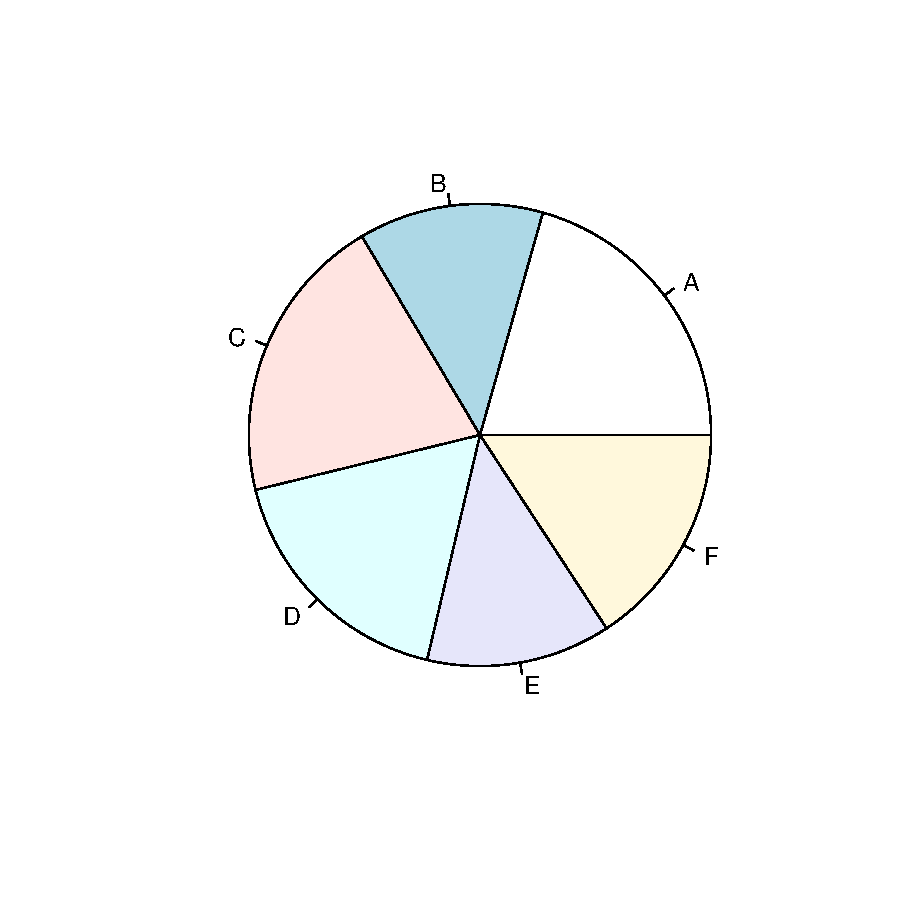
\includegraphics{lect_main-006}

Note that there is no sorting here. Can you easily order the slices
by visual inspection,
i.e., which major has the largest number/percentage of admissions,
which is second, third, etc.?

A better representation
is to sort the data from largest to smallest and then plot
the slices in clockwise direction, starting with the
largest slice at 90$^\circ$.

\begin{Schunk}
\begin{Sinput}
> pie(sort(apply(UCBAdmissions, 3, sum), decreasing = TRUE), 
+     clockwise = TRUE,
+     main = "UC Berkley Admissions by Major")
\end{Sinput}
\end{Schunk}
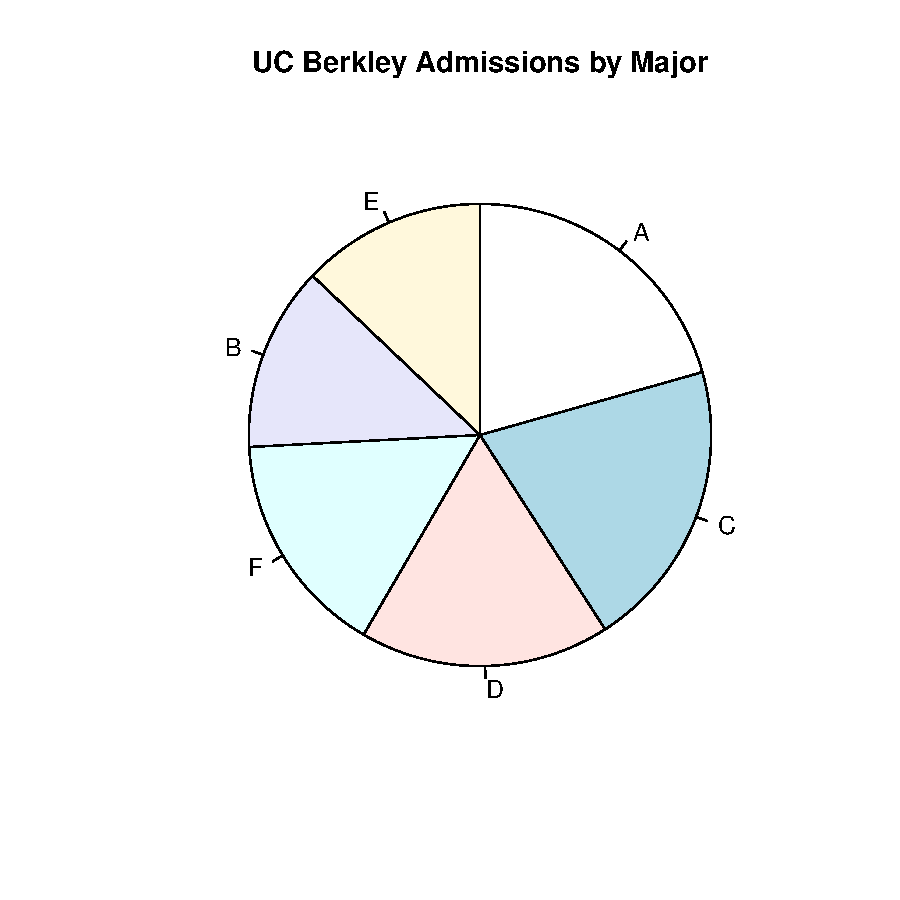
\includegraphics{lect_main-007}

This is somewhat better, but still not perfect. The R help page for pie charts
indicates:
\begin{quotation}
``Pie charts are a very bad way of displaying information. The eye is good 
at judging linear measures and bad at judging relative areas. A bar chart or 
dot chart is a preferable way of displaying this type of data.''
\end{quotation}

Moreover, \cite{Cle85}, p.~264, states: 
\begin{quotation}
``Data that can be shown by pie charts always can be shown by a dot chart. 
This means that judgements of position along a common scale can 
be made instead of the less accurate angle judgements.''
\end{quotation}


{\it ggplot2} allows to draw pie charts, but it is not very supportive.
The help  page for \verb|coord_polar| states:
\begin{quotation}
NOTE: Use these plots with caution - polar coordinates has
major perceptual problems.  The main point of these examples is
to demonstrate how these common plots can be described in the
grammar.  Use with EXTREME caution.
\end{quotation}


\begin{Schunk}
\begin{Sinput}
> library(ggplot2)
> UCBtable <- apply(UCBAdmissions, 3, sum)
> UCBdf <- data.frame(Department = as.factor(names(UCBtable)),
+                     Applicants = UCBtable)
> UCBdf
\end{Sinput}
\begin{Soutput}
  Department Applicants
A          A        933
B          B        585
C          C        918
D          D        792
E          E        584
F          F        714
\end{Soutput}
\begin{Sinput}
> # stacked bar chart
> bp <- ggplot(UCBdf, aes(x = "", y = Applicants, fill = Department)) + 
+   geom_bar(width = 1, stat = "identity")
> bp
\end{Sinput}
\end{Schunk}
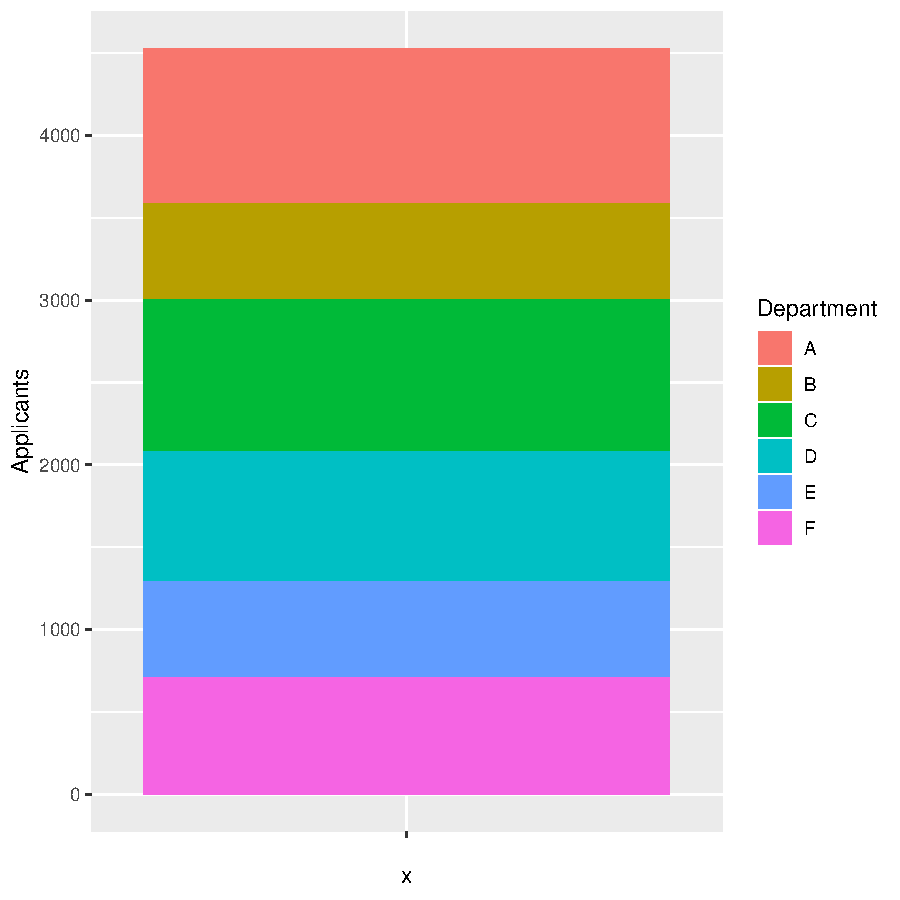
\includegraphics{lect_main-008}

\begin{Schunk}
\begin{Sinput}
> # pie chart
> pie <- bp + coord_polar(theta = "y")
> pie
\end{Sinput}
\end{Schunk}
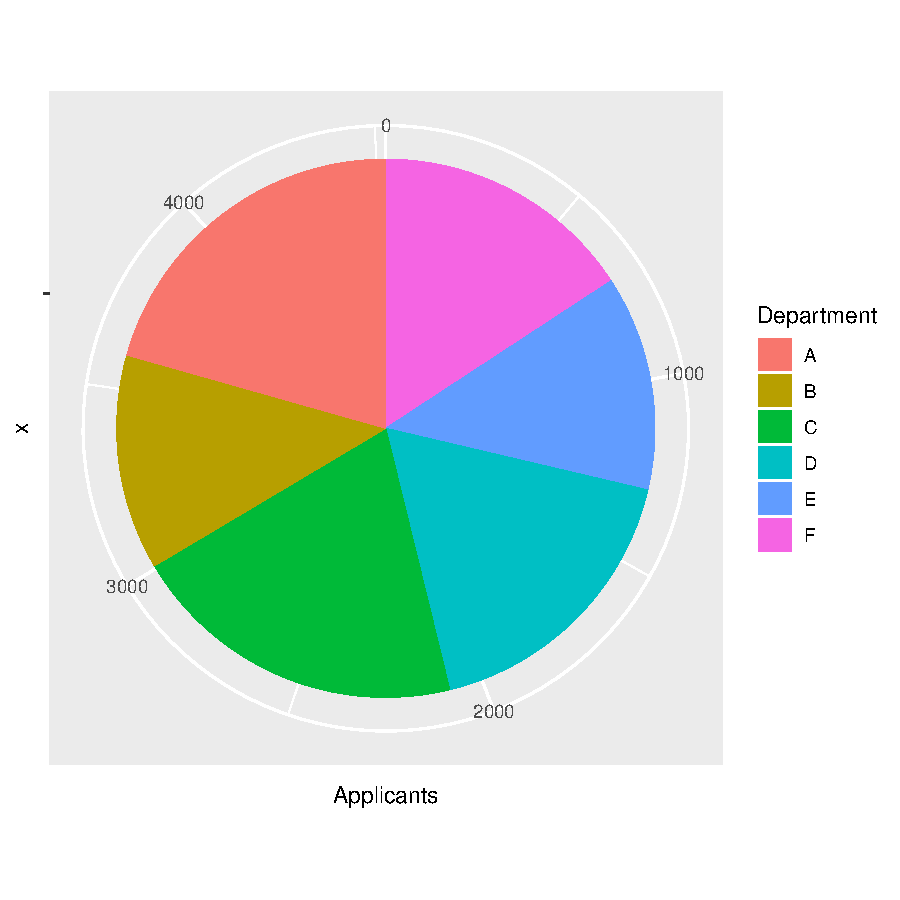
\includegraphics{lect_main-009}

\begin{Schunk}
\begin{Sinput}
> # modified pie chart
> pie <- ggplot(UCBdf, aes(x = "", y = Applicants, fill = Department)) + 
+   geom_bar(width = 1, stat = "identity") + 
+   coord_polar(theta = "y", start = 0, direction = -1) +
+   theme_void() +
+   ggtitle("UC Berkley Admissions by Major") +
+   theme(plot.title = element_text(hjust = 0.5, vjust = -10))
> pie
\end{Sinput}
\end{Schunk}
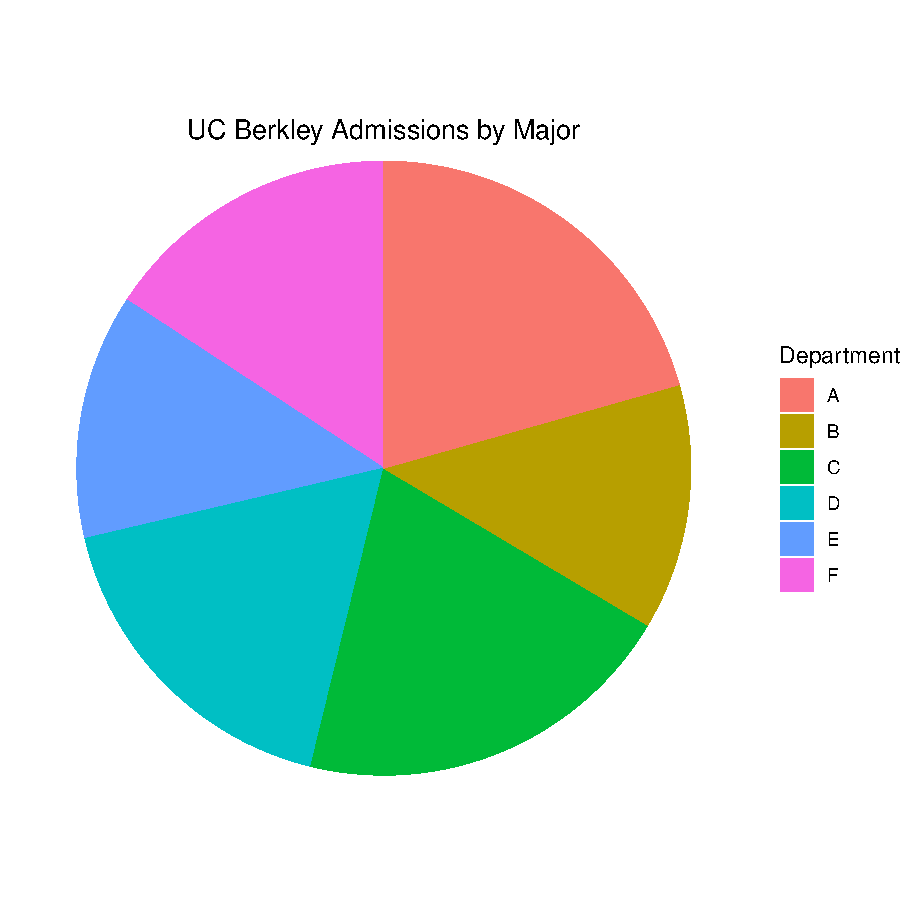
\includegraphics{lect_main-010}

\begin{Schunk}
\begin{Sinput}
> # modified pie chart, sorted from largest to smallest segment
> UCBdfsort <- UCBdf
> UCBdfsort$Department
\end{Sinput}
\begin{Soutput}
[1] A B C D E F
Levels: A B C D E F
\end{Soutput}
\begin{Sinput}
> UCBdfsort$Department <- factor(UCBdfsort$Department, 
+                                levels = UCBdfsort$Department[order(-UCBdfsort$Applicants)])
> UCBdfsort
\end{Sinput}
\begin{Soutput}
  Department Applicants
A          A        933
B          B        585
C          C        918
D          D        792
E          E        584
F          F        714
\end{Soutput}
\begin{Sinput}
> UCBdfsort$Department
\end{Sinput}
\begin{Soutput}
[1] A B C D E F
Levels: A C D F B E
\end{Soutput}
\begin{Sinput}
> pie <- ggplot(UCBdfsort, aes(x = "", y = Applicants, fill = Department)) + 
+   geom_bar(width = 1, stat = "identity") + 
+   coord_polar(theta = "y", start = 0, direction = -1) +
+   theme_void() +
+   ggtitle("UC Berkley Admissions by Major") +
+   theme(plot.title = element_text(hjust = 0.5, vjust = -10))
> pie
\end{Sinput}
\end{Schunk}
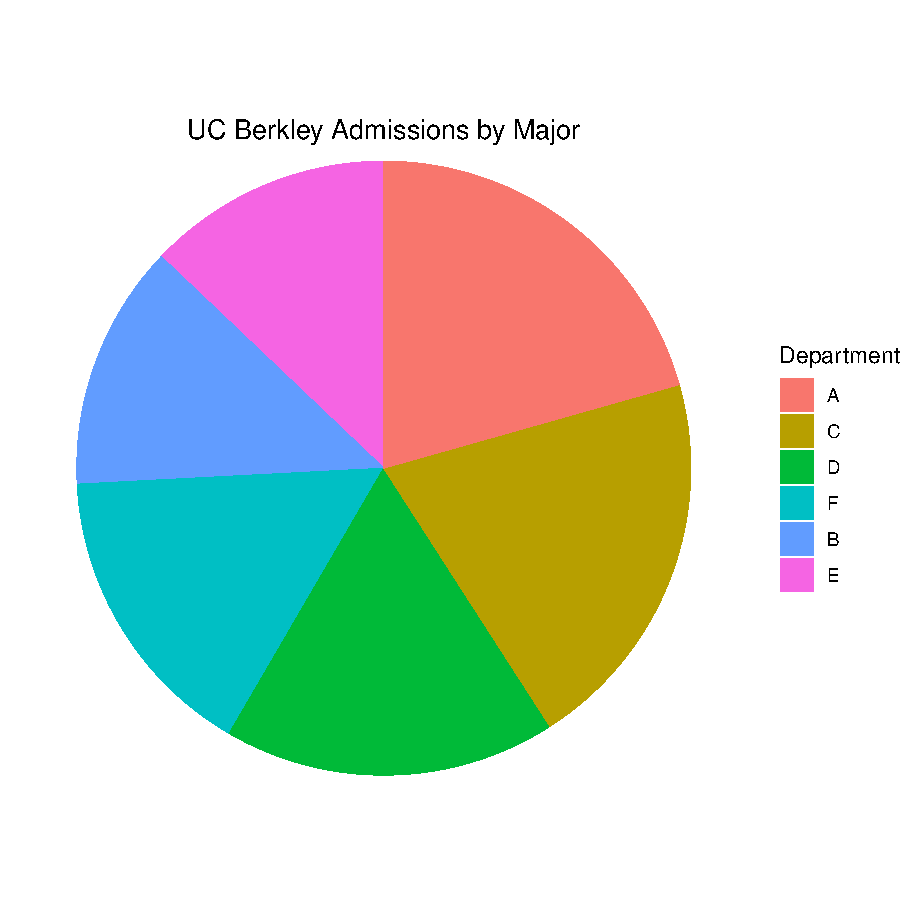
\includegraphics{lect_main-011}

If you further want to adjust your pie chart via {\it ggplot2}, see the
\url{http://www.dxbydt.com/bars-pies-using-ggplot2/} 
web page for additional suggestions.


\newpage


And what about the extremely popular 3D--pie charts that often can be
found in business reports and the media? The answer is 
a clear {\bf Don't.}

\cite{WWPJH96}, p.~70, provide a striking example why not to
use 3D--pie charts. Guess the percentages associated
with the four different areas:

%\begin{figure}[h]
%\centering{\includegraphics[width=4.0in]{Scans//Wallgren_p70_FigG.jpg}}
%\caption{\label{Wallgren_p70_FigG}
%\cite{WWPJH96}, p.~70, Figure~G.
%}
%\end{figure}

And here is the answer:

\if\jsprivatechfour 1

%\begin{figure}[h]
%\centering{\includegraphics[width=4.0in]{Scans//Wallgren_p70_FigF.jpg}}
%\caption{\label{Wallgren_p70_FigF}
%\cite{WWPJH96}, p.~70, Figure~F.
%}
%\end{figure}

\else
{\bf Additional details will be provided after class.}
\fi


\newpage


\subsubsection{Bar Charts}


The R help page for barplot indicates:
\begin{quotation}
``Creates a bar plot with vertical or horizontal bars.''
\end{quotation}


\begin{Schunk}
\begin{Sinput}
> UCBAd <- margin.table(UCBAdmissions, 1:2)
> UCBAd
\end{Sinput}
\begin{Soutput}
          Gender
Admit      Male Female
  Admitted 1198    557
  Rejected 1493   1278
\end{Soutput}
\begin{Sinput}
> barplot(UCBAd, legend.text = TRUE)
\end{Sinput}
\end{Schunk}
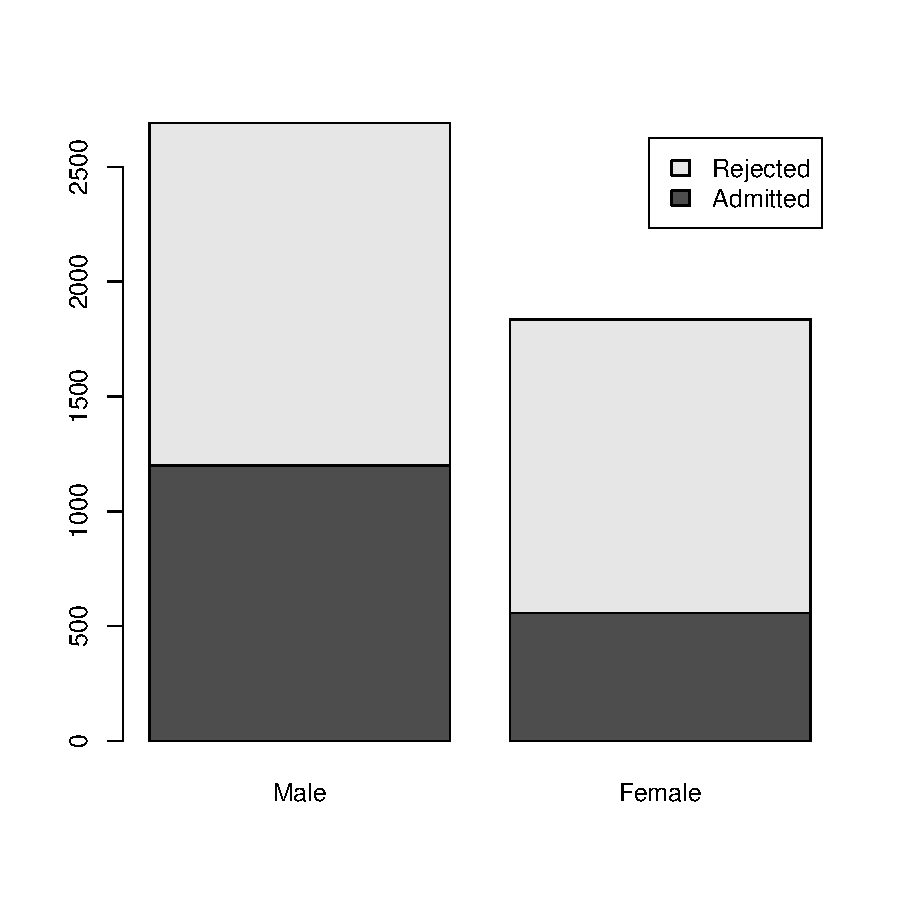
\includegraphics{lect_main-012}

\begin{Schunk}
\begin{Sinput}
> barplot(UCBAd, legend.text = TRUE, beside = TRUE)
\end{Sinput}
\end{Schunk}
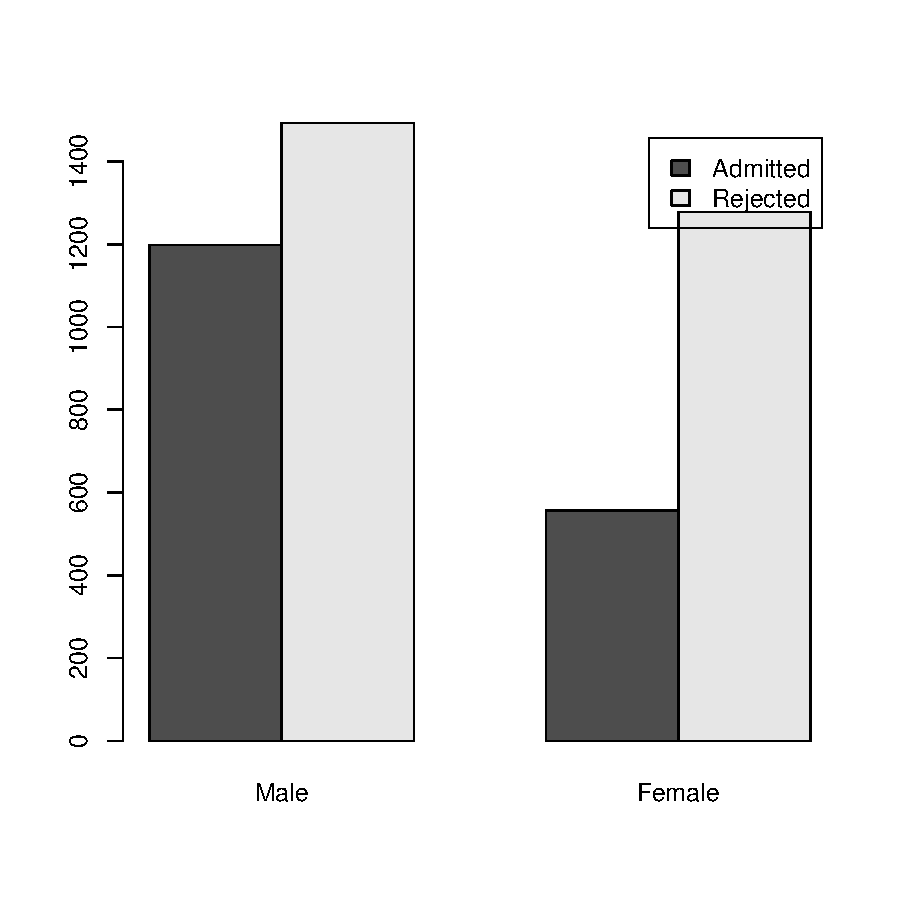
\includegraphics{lect_main-013}

The following commands create (divided) bar charts that show
the percentage admitted/rejected for each gender.

\begin{Schunk}
\begin{Sinput}
> barplot(UCBAd / rbind(margin.table(UCBAd, 2), margin.table(UCBAd, 2)), 
+   legend.text = TRUE)
\end{Sinput}
\end{Schunk}
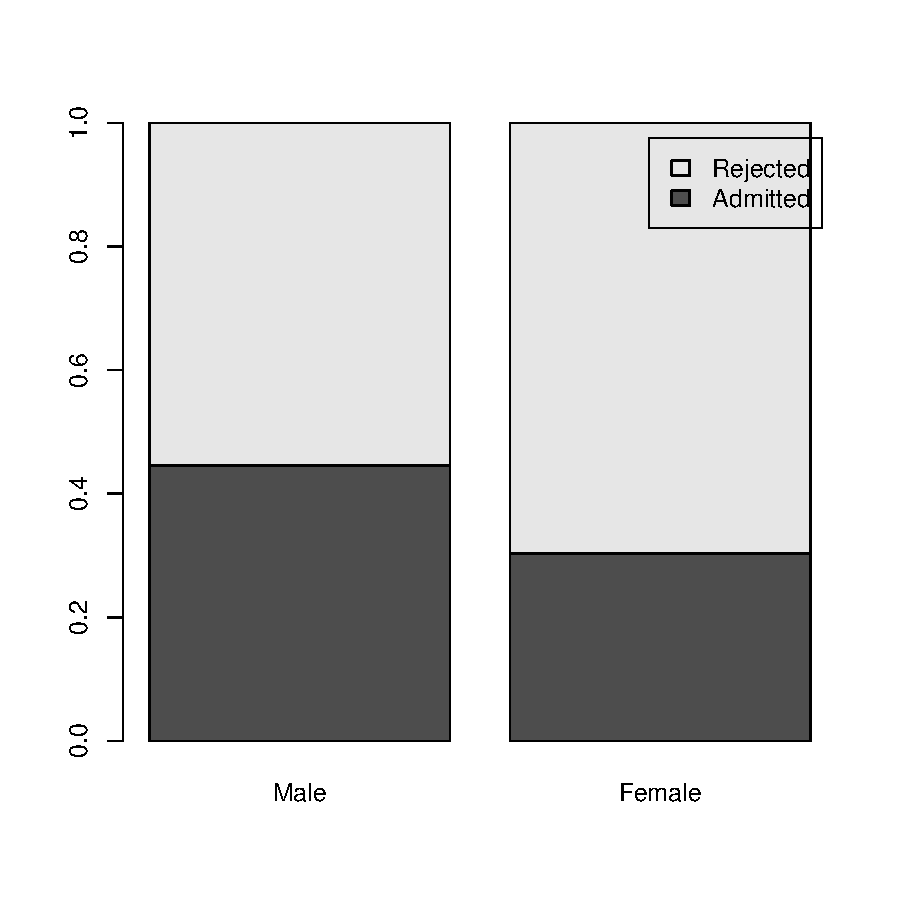
\includegraphics{lect_main-014}

\begin{Schunk}
\begin{Sinput}
> barplot(UCBAd / rbind(margin.table(UCBAd, 2), margin.table(UCBAd, 2)), 
+   legend.text = TRUE, beside = TRUE)
\end{Sinput}
\end{Schunk}
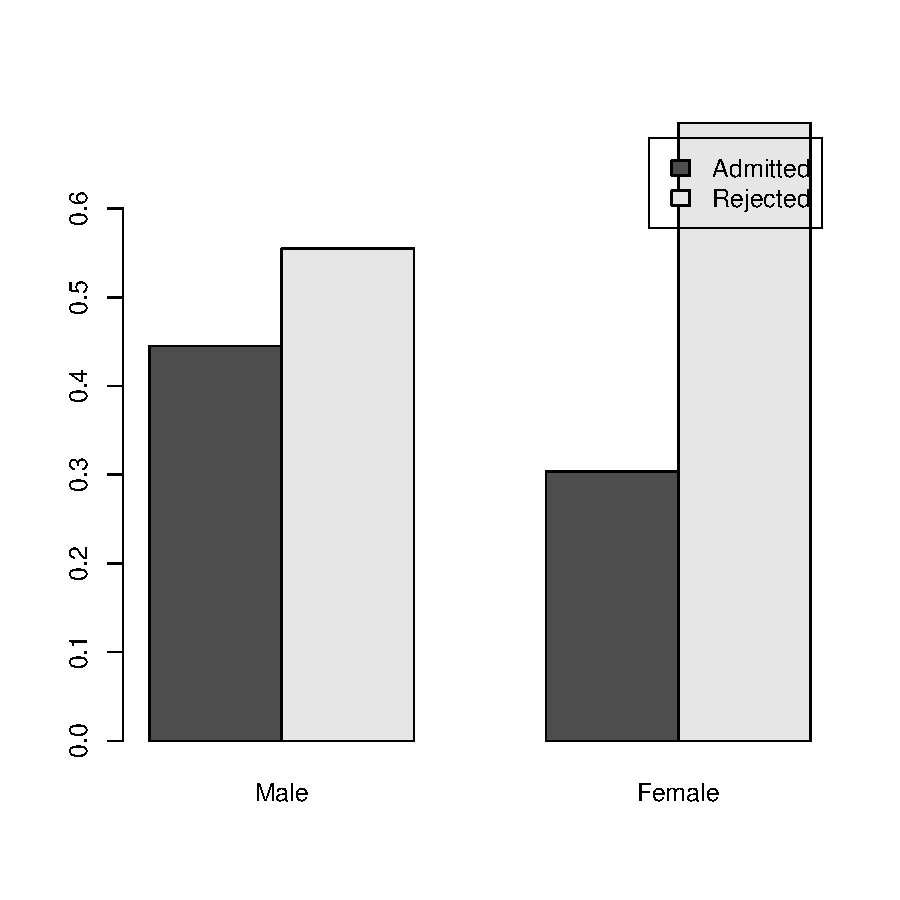
\includegraphics{lect_main-015}


Let's try a few more bar charts with ggplot2. Thanks to Johnny Hong for 
posting these examples at \url{http://jcyhong.github.io/ggplot_demo.html}:

\begin{Schunk}
\begin{Sinput}
> library(ggplot2)
> library(plyr)
> library(gridExtra)
> library(grid)
> UCBdt <- as.data.frame(UCBAdmissions)
> overall <- ddply(UCBdt, .(Gender), function(gender) {
+   temp <- c(sum(gender[gender$Admit == "Admitted", "Freq"]), 
+             sum(gender[gender$Admit == "Rejected", "Freq"])) / sum(gender$Freq)
+   names(temp) <- c("Admitted", "Rejected")
+   temp
+ })
> overall
\end{Sinput}
\begin{Soutput}
  Gender  Admitted  Rejected
1   Male 0.4451877 0.5548123
2 Female 0.3035422 0.6964578
\end{Soutput}
\begin{Sinput}
> departmentwise <- ddply(UCBdt, .(Gender, Dept), function(gender) {
+   temp <- gender$Freq / sum(gender$Freq)
+   names(temp) <- c("Admitted", "Rejected")
+   temp
+ })
> departmentwise
\end{Sinput}
\begin{Soutput}
   Gender Dept   Admitted  Rejected
1    Male    A 0.62060606 0.3793939
2    Male    B 0.63035714 0.3696429
3    Male    C 0.36923077 0.6307692
4    Male    D 0.33093525 0.6690647
5    Male    E 0.27748691 0.7225131
6    Male    F 0.05898123 0.9410188
7  Female    A 0.82407407 0.1759259
8  Female    B 0.68000000 0.3200000
9  Female    C 0.34064081 0.6593592
10 Female    D 0.34933333 0.6506667
11 Female    E 0.23918575 0.7608142
12 Female    F 0.07038123 0.9296188
\end{Soutput}
\begin{Sinput}
> # A barplot for overall admission percentage for each gender.
> p1 <- ggplot(data = overall, aes(x = Gender, y = Admitted, width = 0.2))
> p1 <- p1 + geom_bar(stat = "identity") + 
+   ggtitle("Overall admission percentage") + 
+   ylim(0, 0.5) 
> p1
\end{Sinput}
\end{Schunk}
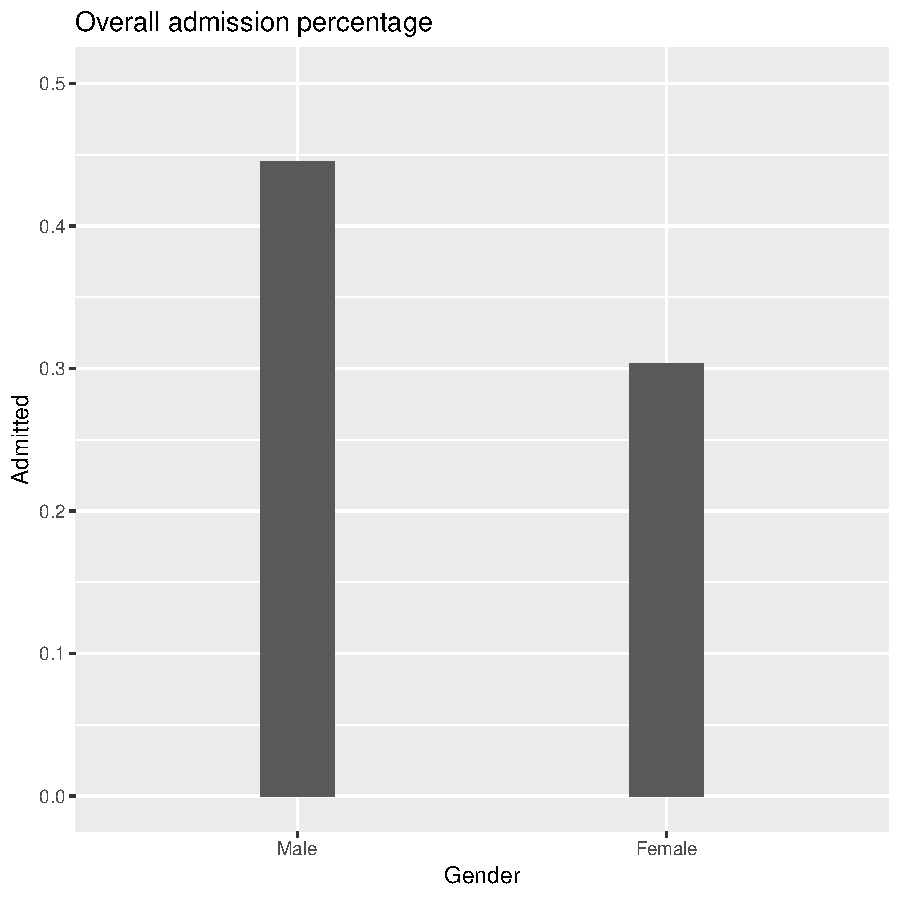
\includegraphics{lect_main-016}

\begin{Schunk}
\begin{Sinput}
> # A 1x6 panel of barplots, each of which represents the 
> # number of admitted students for a department
> p2 <- ggplot(data = UCBdt[UCBdt$Admit == "Admitted", ], aes(x = Gender, y = Freq))
> p2 <- p2 + geom_bar(stat = "identity") + 
+   facet_grid(. ~ Dept) +
+   ggtitle("Number of admitted students\nfor each department") + 
+   theme(axis.text.x = element_text(angle = 90, hjust = 1)) 
> p2
\end{Sinput}
\end{Schunk}
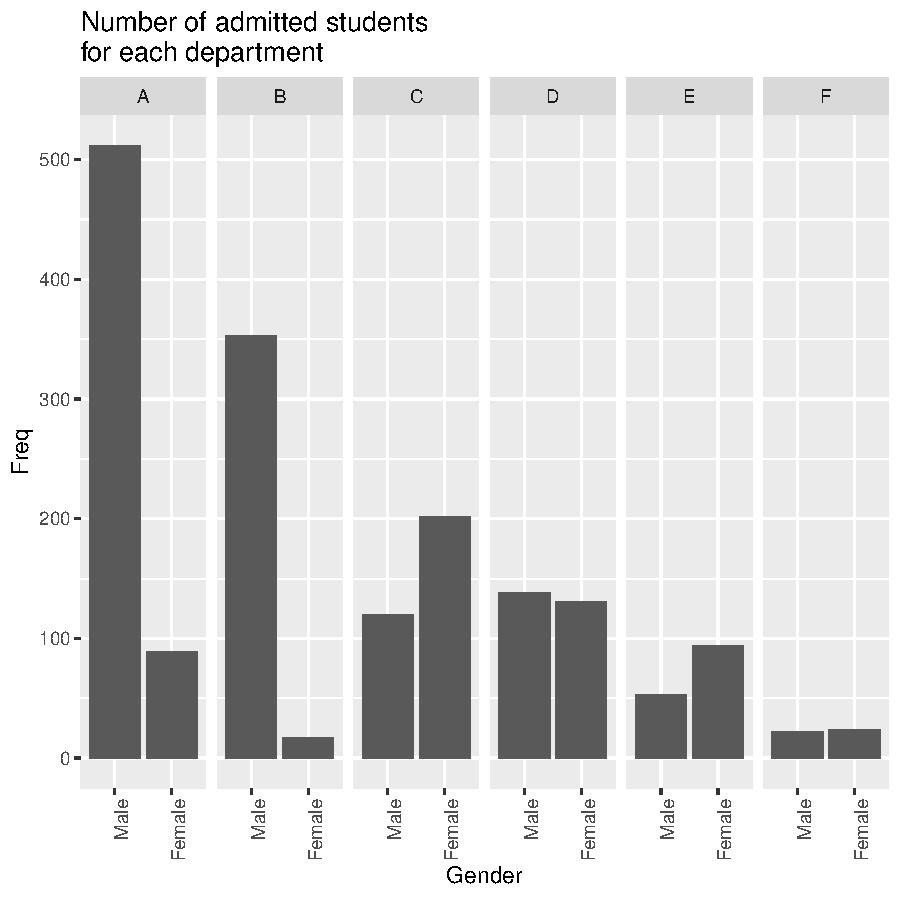
\includegraphics{lect_main-017}

\begin{Schunk}
\begin{Sinput}
> # A 1x6 panel of barplots, each of which represents the 
> # admission percentage for a department
> p3 <- ggplot(data = departmentwise, aes(x = Gender, y = Admitted))
> p3 <- p3 + geom_bar(stat = "identity") + 
+   facet_grid(. ~ Dept) + 
+   ylim(0, 1) +
+   ggtitle("Admission percentage\nfor each department") + 
+   theme(axis.text.x = element_text(angle = 90, hjust = 1))
> p3
\end{Sinput}
\end{Schunk}
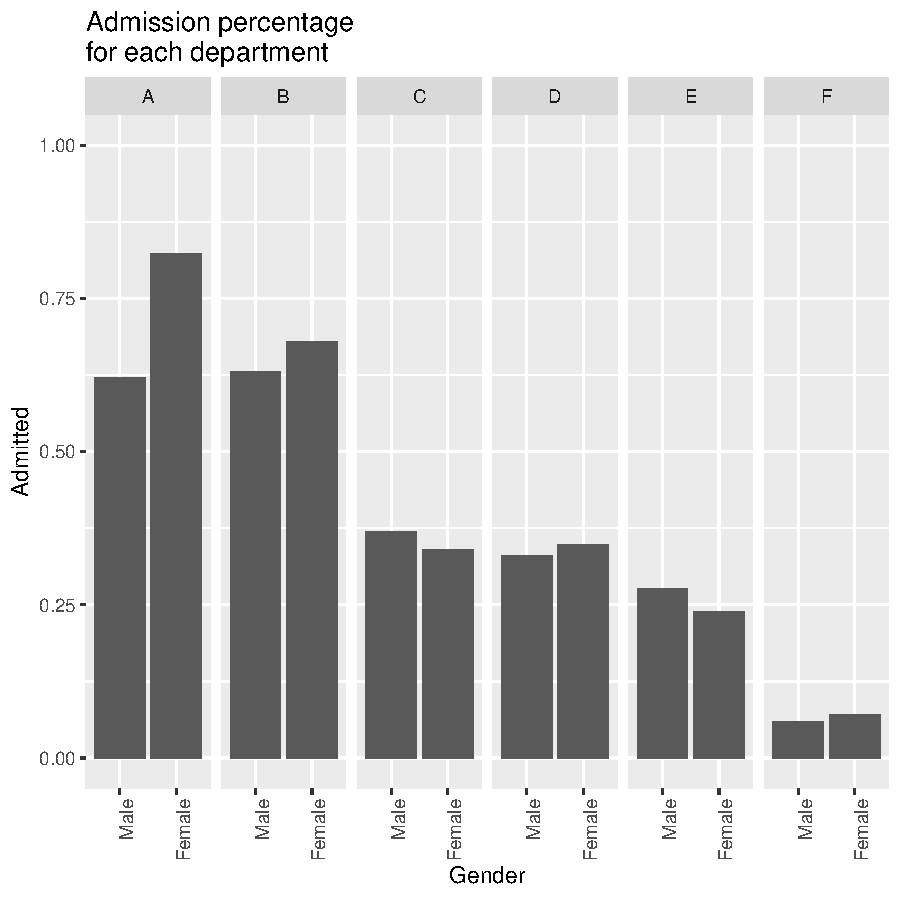
\includegraphics{lect_main-018}

\begin{Schunk}
\begin{Sinput}
> # A 1x6 panel of barplots, each of which represents the 
> # number of applicants for a department
> p4 <- ggplot(data = UCBdt, aes(x = Gender, y = Freq))
> p4 <- p4 + geom_bar(stat = "identity") + 
+   facet_grid(. ~ Dept) + 
+   ggtitle("Number of Applicants\nfor each department") + 
+   theme(axis.text.x = element_text(angle = 90, hjust = 1))
> p4
\end{Sinput}
\end{Schunk}
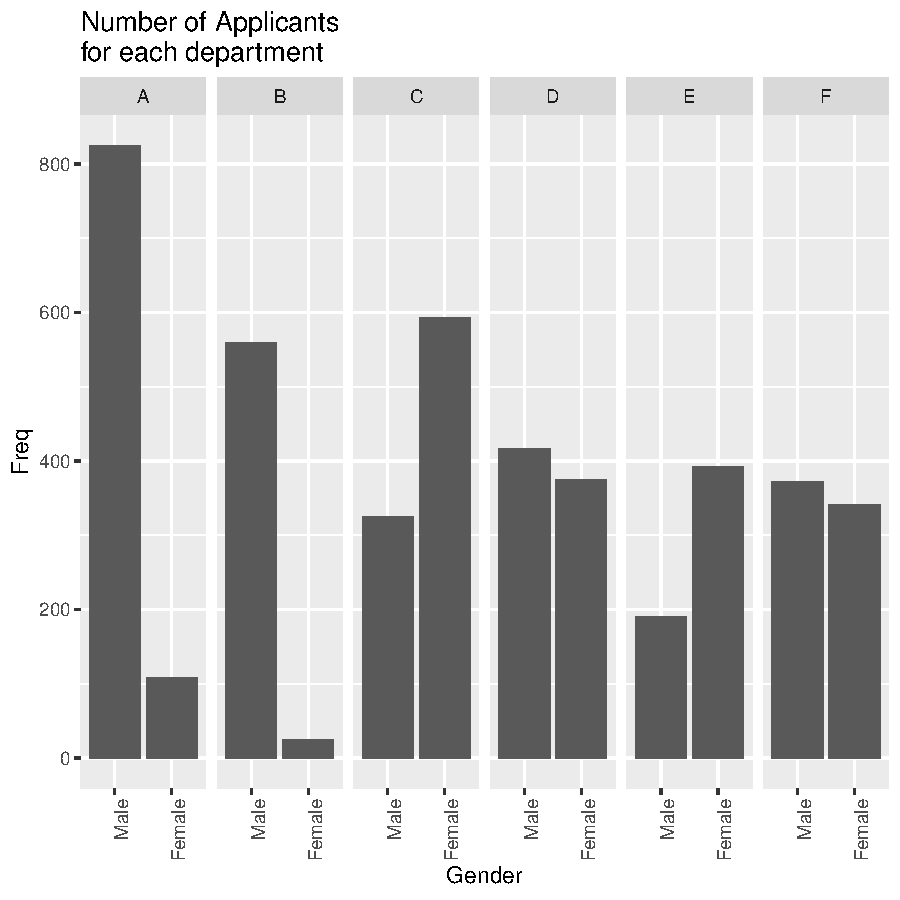
\includegraphics{lect_main-019}

\begin{Schunk}
\begin{Sinput}
> # Arrange the four plots on a page
> grid.arrange(p1, p2, p3, p4, nrow = 2, 
+              top = textGrob("Simpson's Paradox: UC Berkeley 1973 Admissions", 
+                             gp = gpar(fontsize = 15)))
\end{Sinput}
\end{Schunk}
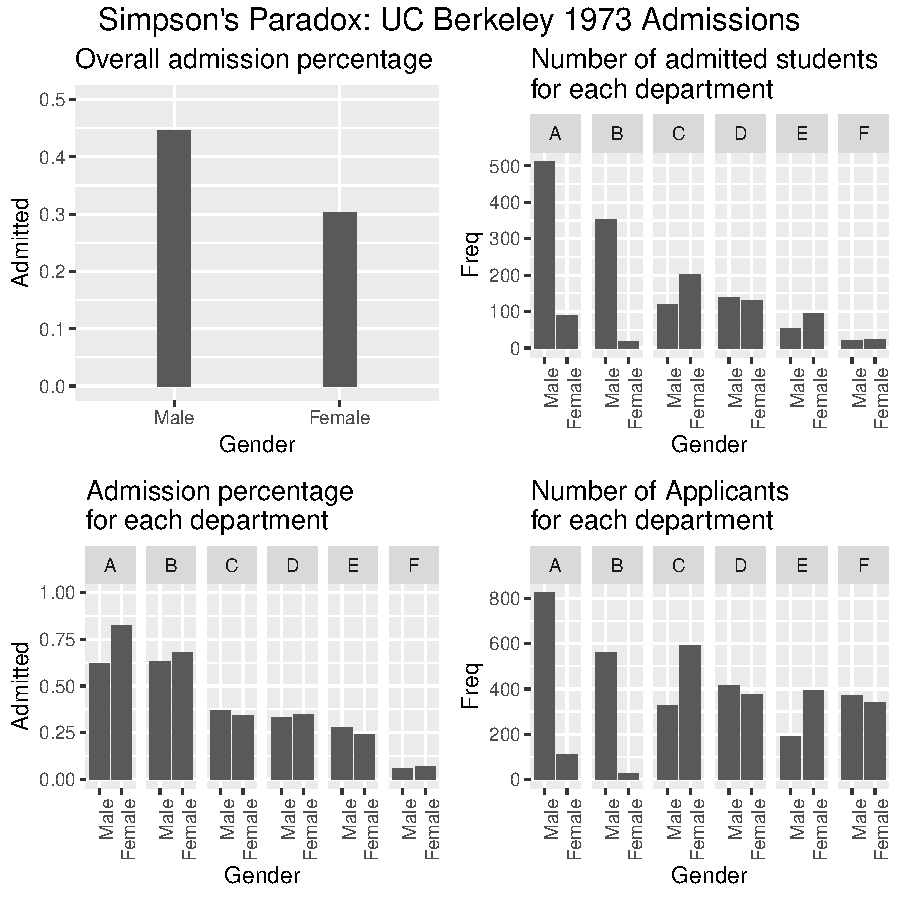
\includegraphics{lect_main-020}


Blogger ``wszafranski'' provided further suggestions how to modify bar charts in ggplot2
at \url{https://www.r-bloggers.com/make-a-bar-plot-with-ggplot/}.
Let's apply some of these to the previously created bar charts and compare them side-by-side.

\begin{Schunk}
\begin{Sinput}
> # A 1x6 panel of barplots, each of which represents the 
> # number of applicants for a department;
> # moreover, make a distinction between Admitted & Rejected
> p5 <- ggplot(data = UCBdt, aes(x = Gender, y = Freq))
> p5 <- p5 + geom_bar(stat = "identity", aes(fill = Admit)) + 
+   facet_grid(. ~ Dept) + 
+   ggtitle("Number of Applicants\nfor each department") + 
+   theme(axis.text.x = element_text(angle = 90, hjust = 1))
> p5
\end{Sinput}
\end{Schunk}
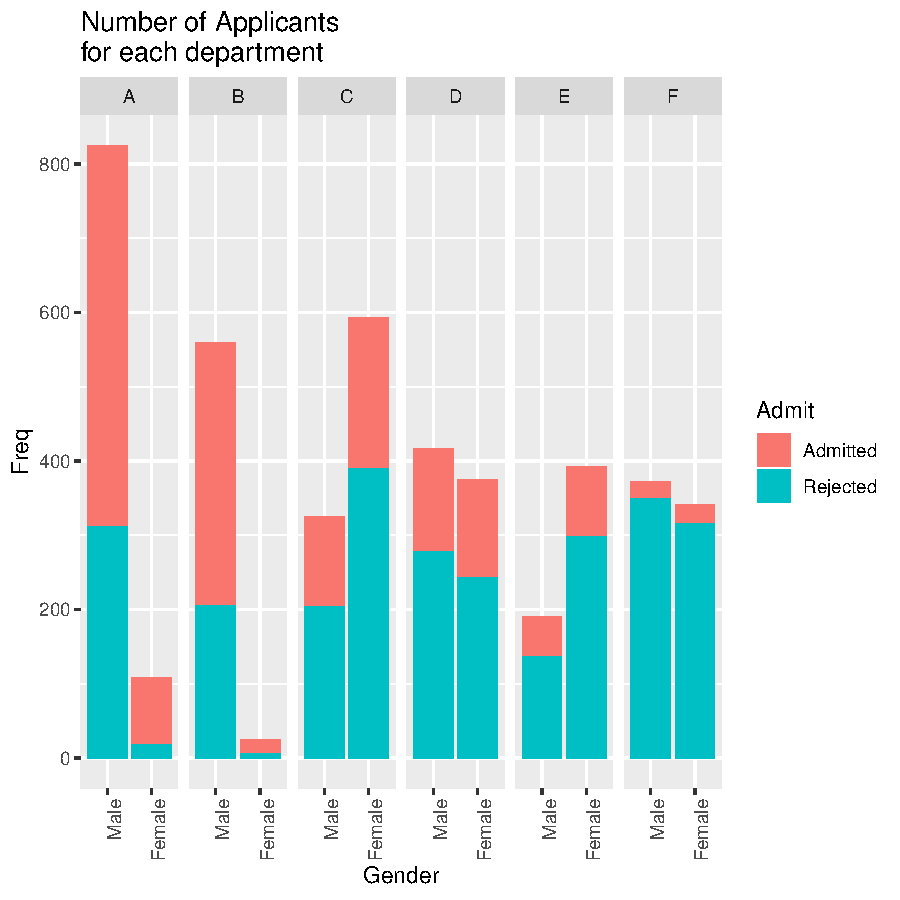
\includegraphics{lect_main-021}

\begin{Schunk}
\begin{Sinput}
> # A 1x6 panel of barplots, each of which represents the 
> # number of applicants for a department;
> # moreover, make a distinction between Admitted & Rejected 
> # and place these bars side-by-side
> p6 <- ggplot(data = UCBdt, aes(x = Gender, y = Freq))
> p6 <- p6 + geom_bar(stat = "identity", aes(fill = Admit), position = "dodge") + 
+   facet_grid(. ~ Dept) + 
+   ggtitle("Number of Applicants\nfor each department") + 
+   theme(axis.text.x = element_text(angle = 90, hjust = 1))
> p6
\end{Sinput}
\end{Schunk}
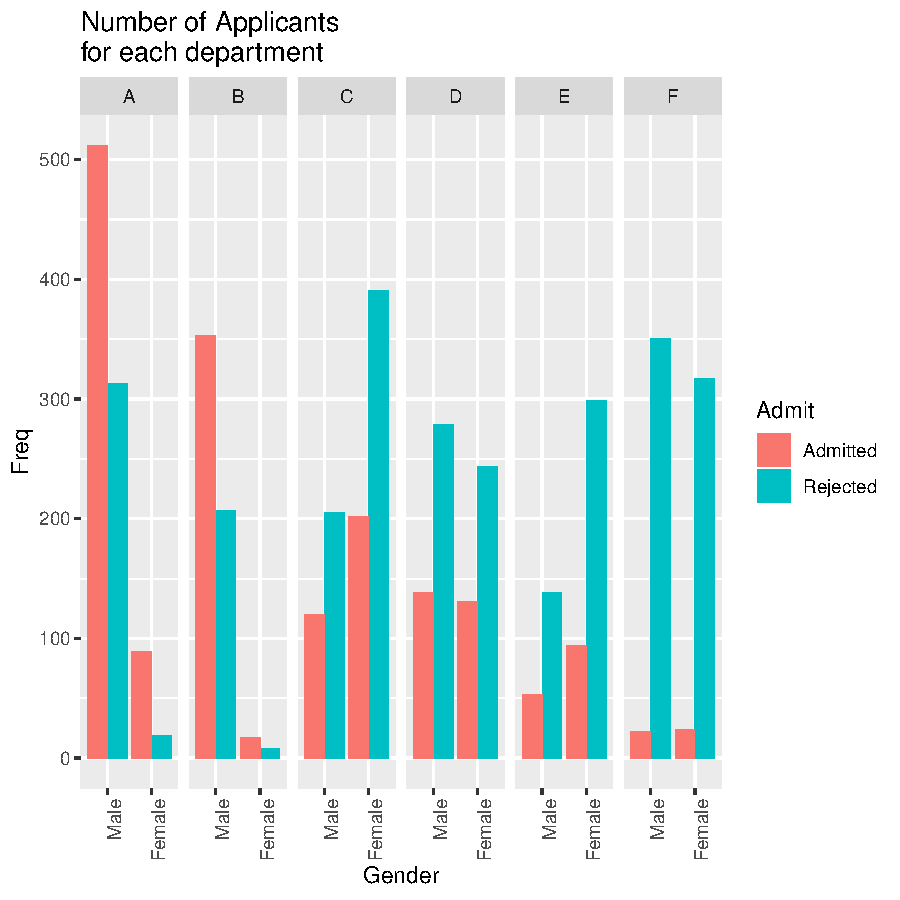
\includegraphics{lect_main-022}

\begin{Schunk}
\begin{Sinput}
> # Arrange the three plots on a page
> grid.arrange(p4, p5, p6, nrow = 2, 
+              top = textGrob("Focus on Admit: UC Berkeley 1973 Admissions", 
+                             gp = gpar(fontsize = 15)))
\end{Sinput}
\end{Schunk}
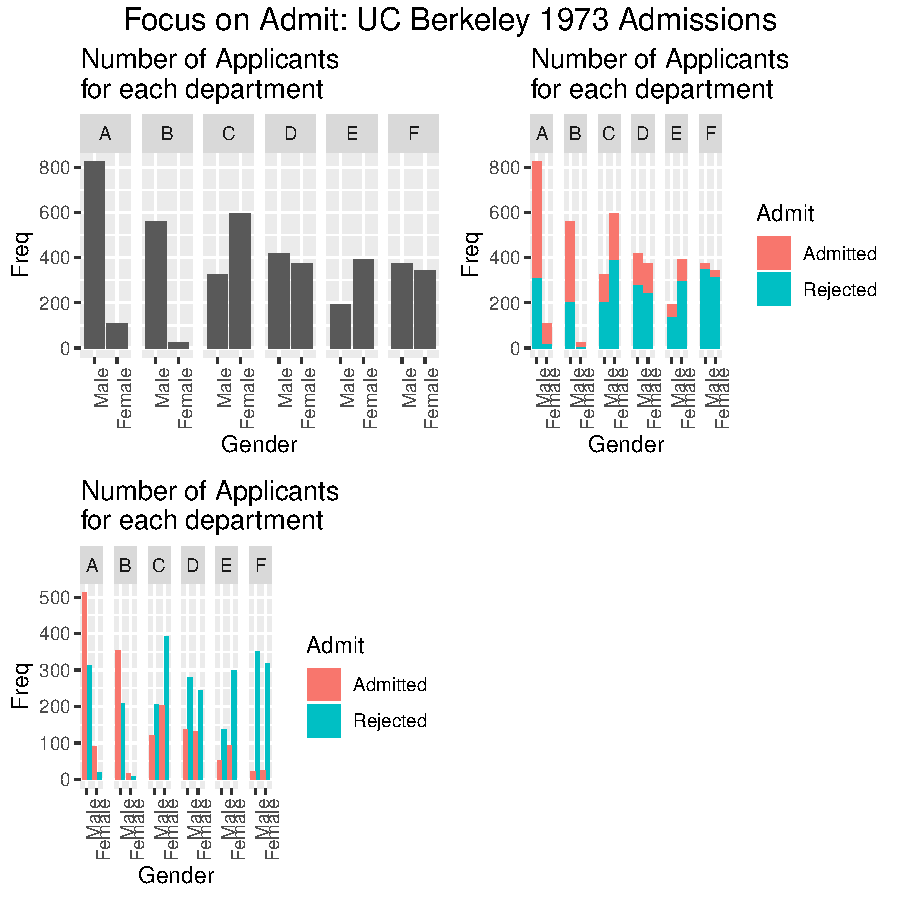
\includegraphics{lect_main-023}


\fbox{\parbox{\textwidth}{
\underline{\bf Warning:} \\
\cite{Cle94}, Section~4.10, ``Pop Charts'', p.~262,
strongly advises against the use of pie charts, divided bar charts, and area charts:
%
\begin{quotation}
Three graphical methods --- pie charts, divided bar charts, and area charts ---
are widely used in mass media and business publications but are used far less
in science and technology. Because of their use, we will call these
graphical methods {\it pop charts}.

Any data that can be encoded by one of these pop charts can also be
encoded by either a dot plot or a multiway dot plot that typically
provides far more efficient pattern perception and
table look--up than the pop--chart encoding. Interestingly, the
better pattern perception results from a detection operation,
a phenomenon that has been missed in previous studies of pop charts.
\end{quotation}
}}


\newpage

Finally, what about 3D bar charts?
\cite{SRH2016ASA} discussed problems with 3D bar charts in detail.
They stated: 
\begin{quotation}
``There are
several reasons that we object to these 3D charts. Our main objection is that most people
are misled by them. They don't know where the value is encoded. In Figure 11 (left), is the
value at the front of the bar as indicated by the arrow on the A bar or is it in the back of the
bar as indicated by the arrow on the B bar? Most readers judge the A bar to be around 0.75
and the B bar to be about 1.75. [$\ldots$] \\
Our second objection to pseudo 3D graphs is that different software programs draw
them differently. PowerPoint is in the same suite of programs as Excel but earlier versions
of PowerPoint did have a default gap depth of zero. Therefore, the usual value of a 3D
bar graph drawn using these versions of PowerPoint was read from the back of the bar.
Figure 12 (left) shows a figure from PowerPoint 2003 (not the same data as in Figures 11).
A number of software programs show the value from the front of the bar as in the arrow
of the A bar in Figure 11 and in Figure 12 (right). Even different versions of the same
software may have different defaults. We find it unacceptable that the way to read a figure
should depend on the software used to draw it. Readers often don't know what software
was used and even if they did, they probably don't know the algorithm used.''
\end{quotation}


\newpage


%\begin{figure}[h]
%\centering{\includegraphics[width=6.0in]{Scans//SRH_2016_Fig11.jpg}}
%\caption{\label{SRH_2016_Fig11}
%\cite{SRH2016ASA}, Figure~11: 
%Many readers are not sure how to read an Excel 3D bar chart (left). An Excel
%2D bar chart is much clearer (right).
%}
%\end{figure}


%\begin{figure}[h]
%\centering{\includegraphics[width=6.0in]{Scans//SRH_2016_Fig12.jpg}}
%\caption{\label{SRH_2016_Fig12}
%\cite{SRH2016ASA}, Figure~12: 
%With PowerPoint 2003 you read from the back of the bar (left). With Presentations
%and Charts you read from the front of the bar (right).
%}
%\end{figure}


\newpage


\subsubsection{Dot Plots / Dot Charts}


The R help page for dotchart indicates:
\begin{quotation}
``Draw a Cleveland dot plot. [$\ldots$] \\
This function is invoked for its side effect, which is to produce two variants 
of dotplots as described in \cite{Cle85}. 
Dot plots are a reasonable substitute for bar plots.''
\end{quotation}


\begin{Schunk}
\begin{Sinput}
> dotchart(UCBAd)
\end{Sinput}
\end{Schunk}
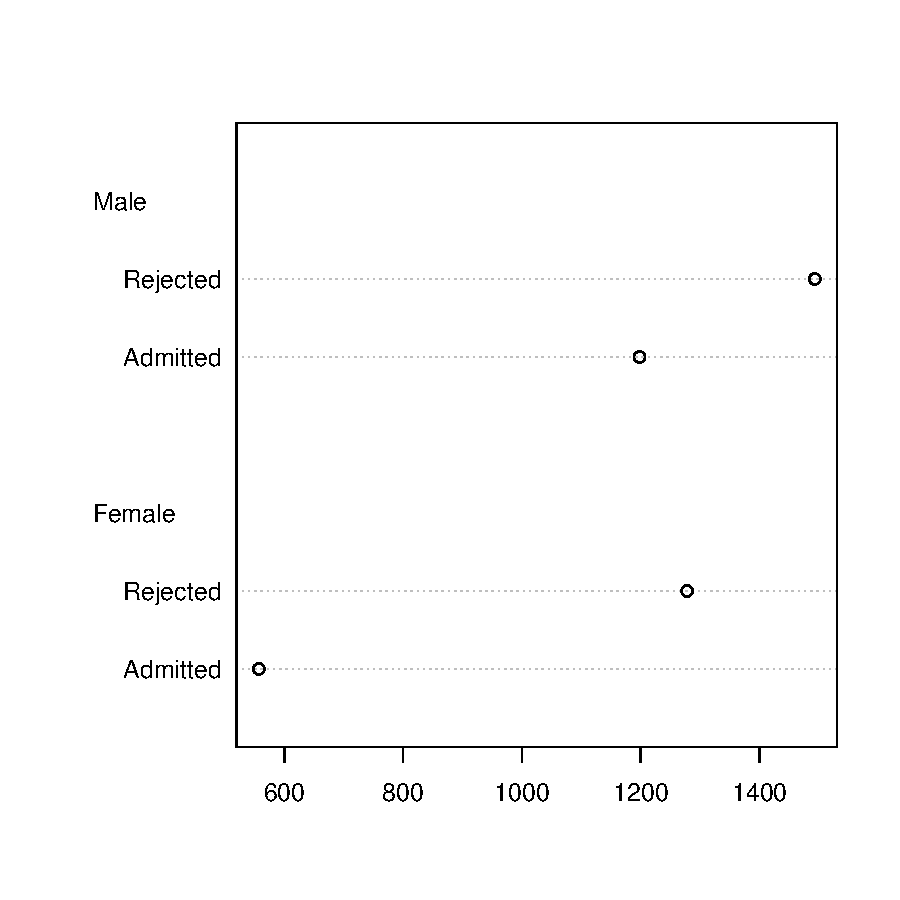
\includegraphics{lect_main-024}

\begin{Schunk}
\begin{Sinput}
> UCBMajor <- margin.table(UCBAdmissions, 2:3)
> dotchart(UCBMajor)
\end{Sinput}
\end{Schunk}
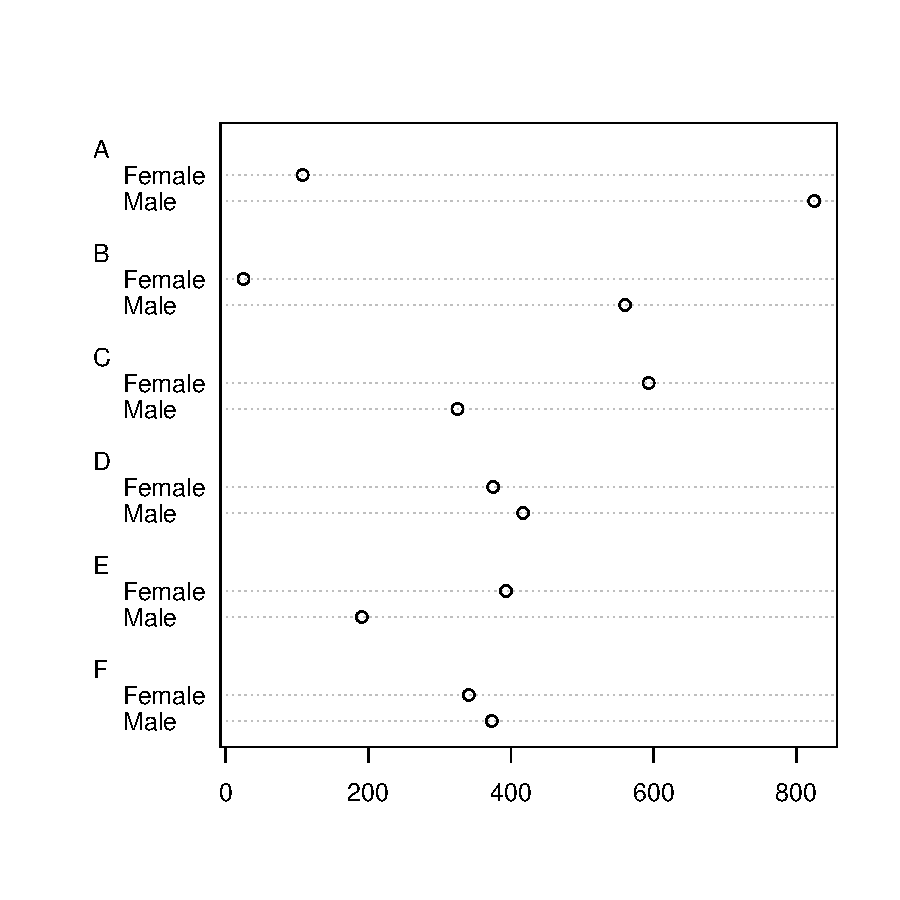
\includegraphics{lect_main-025}

\begin{Schunk}
\begin{Sinput}
> UCBMajorsort <- UCBMajor[, order(UCBMajor[1, ], decreasing = TRUE)]
> dotchart(UCBMajorsort, color = c("purple", "orange"))
\end{Sinput}
\end{Schunk}
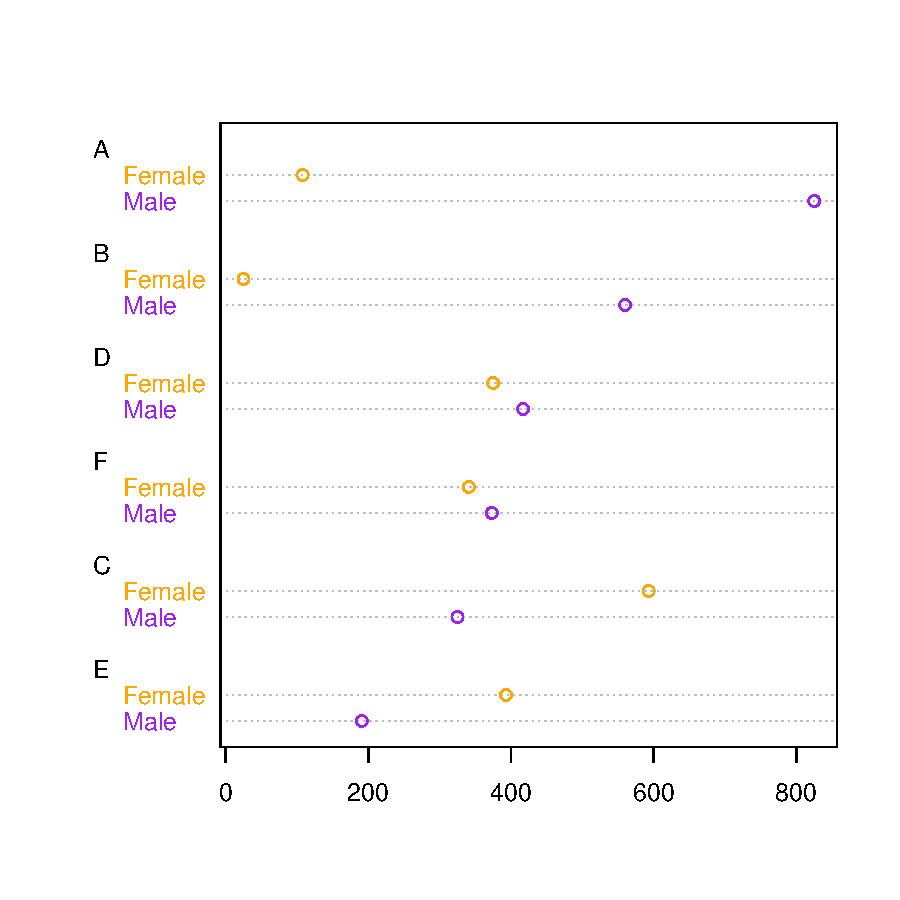
\includegraphics{lect_main-026}


Let's try a few more dot plots with ggplot2. 

\begin{Schunk}
\begin{Sinput}
> library(ggplot2)
> library(plyr)
> library(gridExtra)
> library(grid)
> UCBdt <- as.data.frame(UCBAdmissions)
> overall <- ddply(UCBdt, .(Gender), function(gender) {
+   temp <- c(sum(gender[gender$Admit == "Admitted", "Freq"]), 
+             sum(gender[gender$Admit == "Rejected", "Freq"])) / sum(gender$Freq)
+   names(temp) <- c("Admitted", "Rejected")
+   temp
+ })
> overall
\end{Sinput}
\begin{Soutput}
  Gender  Admitted  Rejected
1   Male 0.4451877 0.5548123
2 Female 0.3035422 0.6964578
\end{Soutput}
\begin{Sinput}
> departmentwise <- ddply(UCBdt, .(Gender, Dept), function(gender) {
+   temp <- gender$Freq / sum(gender$Freq)
+   names(temp) <- c("Admitted", "Rejected")
+   temp
+ })
> departmentwise
\end{Sinput}
\begin{Soutput}
   Gender Dept   Admitted  Rejected
1    Male    A 0.62060606 0.3793939
2    Male    B 0.63035714 0.3696429
3    Male    C 0.36923077 0.6307692
4    Male    D 0.33093525 0.6690647
5    Male    E 0.27748691 0.7225131
6    Male    F 0.05898123 0.9410188
7  Female    A 0.82407407 0.1759259
8  Female    B 0.68000000 0.3200000
9  Female    C 0.34064081 0.6593592
10 Female    D 0.34933333 0.6506667
11 Female    E 0.23918575 0.7608142
12 Female    F 0.07038123 0.9296188
\end{Soutput}
\begin{Sinput}
> # 3 alternative ways for the same graph
> 
> ggplot(data = overall, aes(x = Gender, y = Admitted)) +
+   geom_point()
> # or
> 
> ggplot(data = overall) +
+   geom_point(aes(x = Gender, y = Admitted))
> # or
> 
> qplot(Gender, Admitted, data = overall)
> 
> # Note: qplot is a shortcut that can be used for some graphs in ggplot
\end{Sinput}
\end{Schunk}
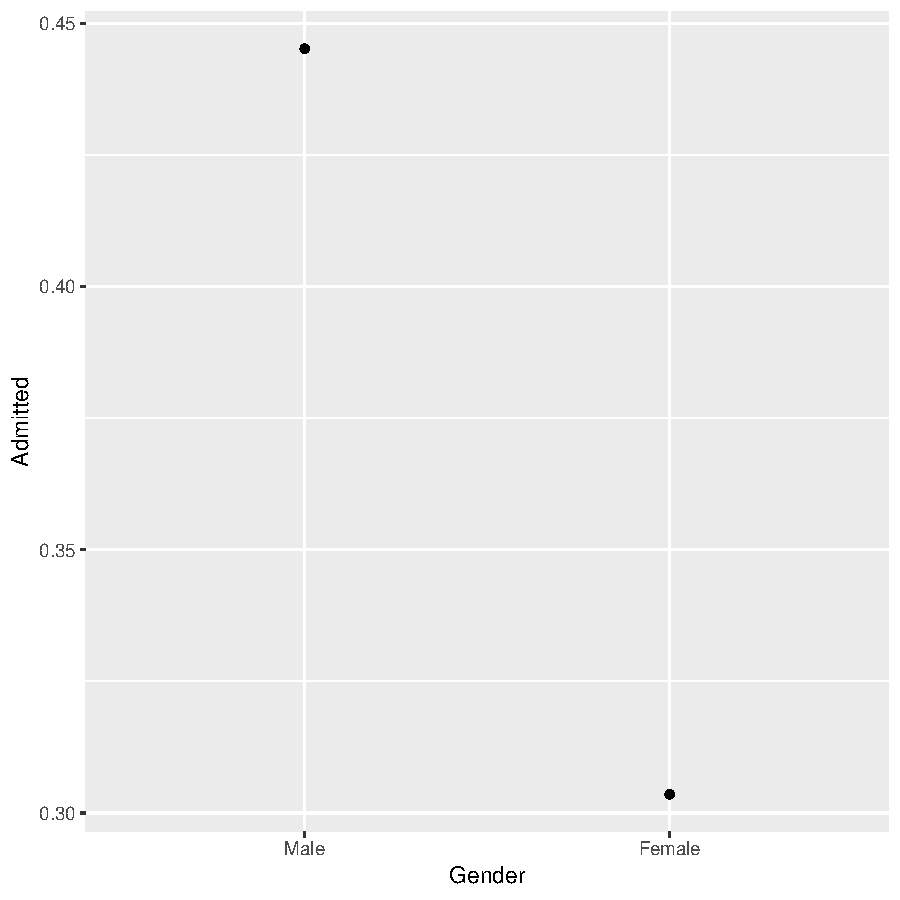
\includegraphics{lect_main-027}

\begin{Schunk}
\begin{Sinput}
> ggplot(data = overall, aes(x = Gender, y = Admitted, colour = Gender)) +
+   geom_point()
> # or
> 
> ggplot(data = overall) +
+   geom_point(aes(x = Gender, y = Admitted, colour = Gender))
> # or
> 
> qplot(Gender, Admitted, data = overall, colour = Gender)
\end{Sinput}
\end{Schunk}
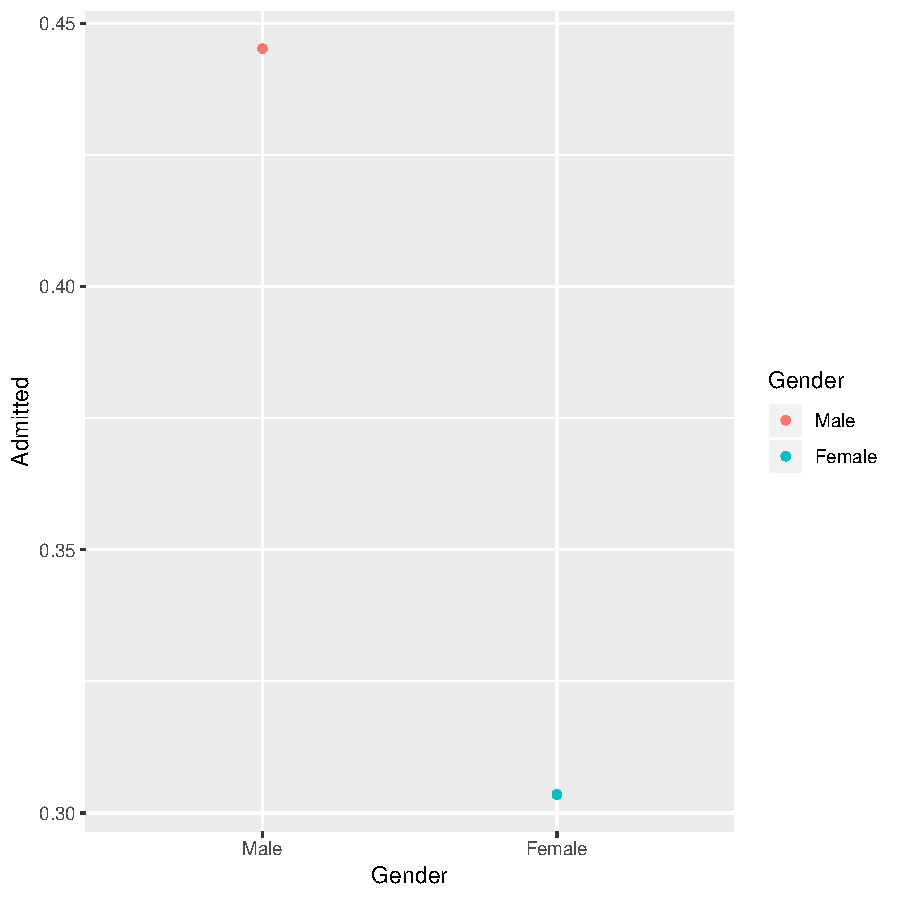
\includegraphics{lect_main-028}

\begin{Schunk}
\begin{Sinput}
> ggplot(data = departmentwise) +
+   geom_point(aes(x = Gender, y = Admitted))
> # or
> 
> qplot(Gender, Admitted, data = departmentwise)
\end{Sinput}
\end{Schunk}
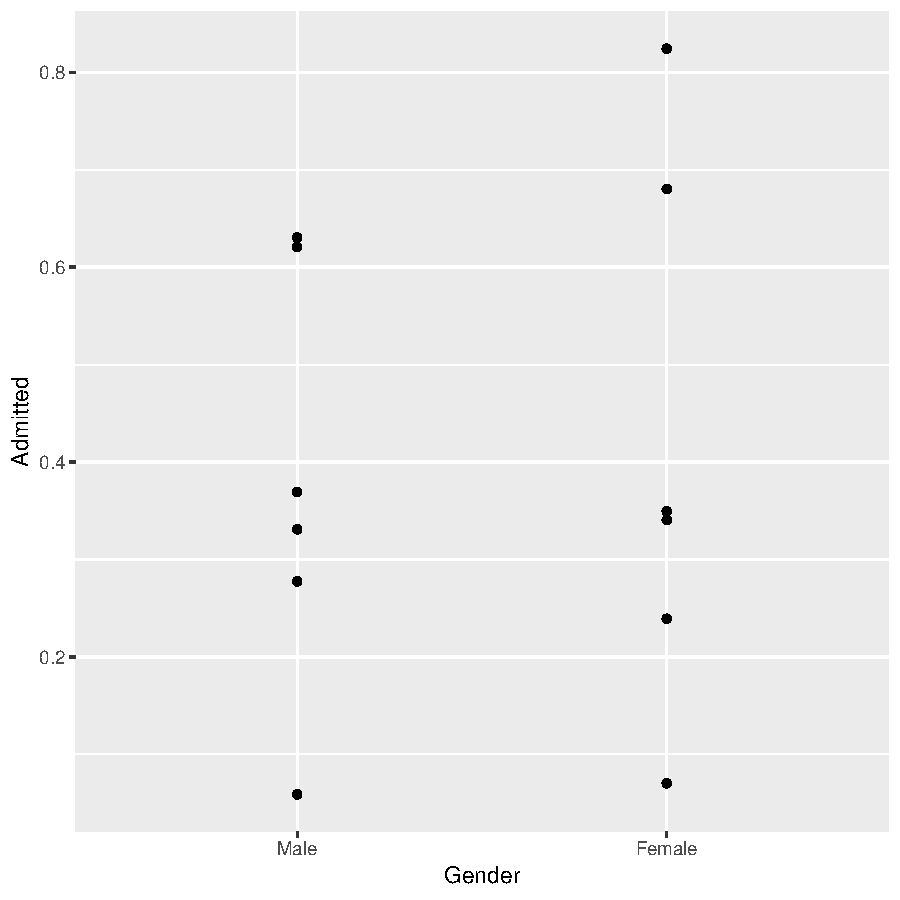
\includegraphics{lect_main-029}

\begin{Schunk}
\begin{Sinput}
> ggplot(data = departmentwise) +
+   geom_point(aes(x = Gender, y = Admitted, colour = Dept))
> # or
> 
> qplot(Gender, Admitted, data = departmentwise, colour = Dept)
\end{Sinput}
\end{Schunk}
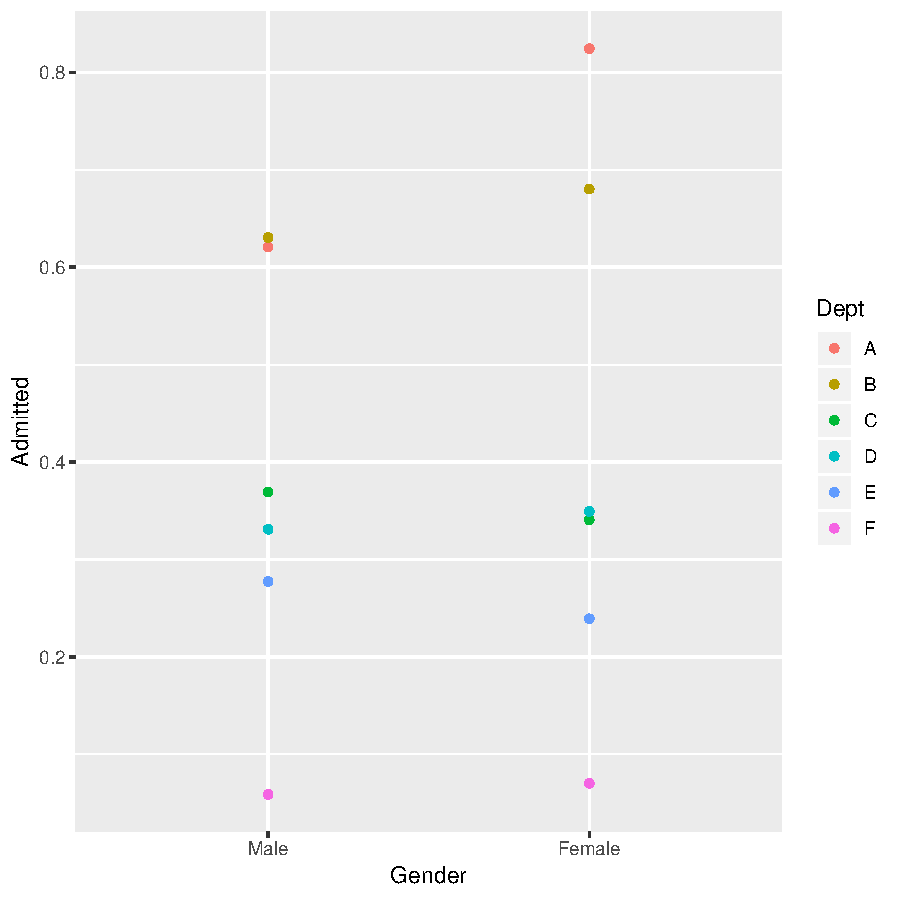
\includegraphics{lect_main-030}

\begin{Schunk}
\begin{Sinput}
> ggplot(data = departmentwise) +
+   geom_point(aes(x = Gender, y = Admitted, colour = Dept)) +
+   facet_grid(~ Dept)
> # or
> 
> qplot(Gender, Admitted, data = departmentwise, colour = Dept) +
+   facet_grid(~ Dept)
\end{Sinput}
\end{Schunk}
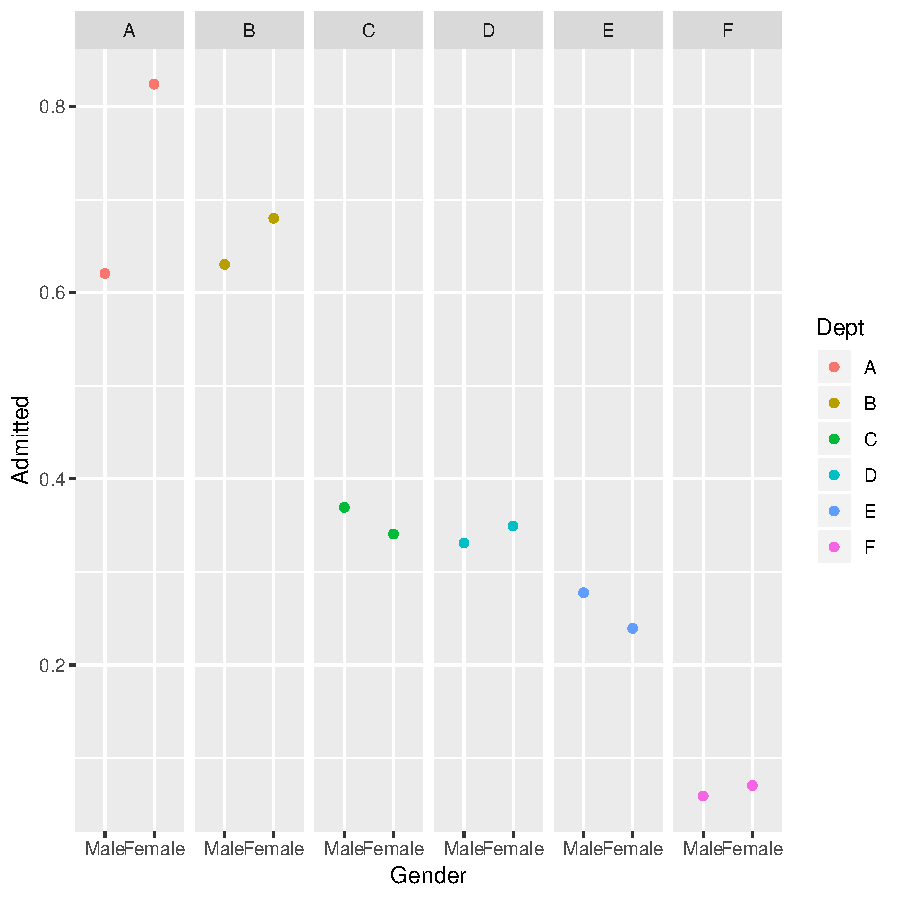
\includegraphics{lect_main-031}

\begin{Schunk}
\begin{Sinput}
> ggplot(data = departmentwise) +
+   geom_point(aes(x = Gender, y = Admitted, colour = Gender)) +
+   facet_grid(~ Dept)
> # or
> 
> qplot(Gender, Admitted, data = departmentwise, colour = Gender) +
+   facet_grid(~ Dept)
\end{Sinput}
\end{Schunk}
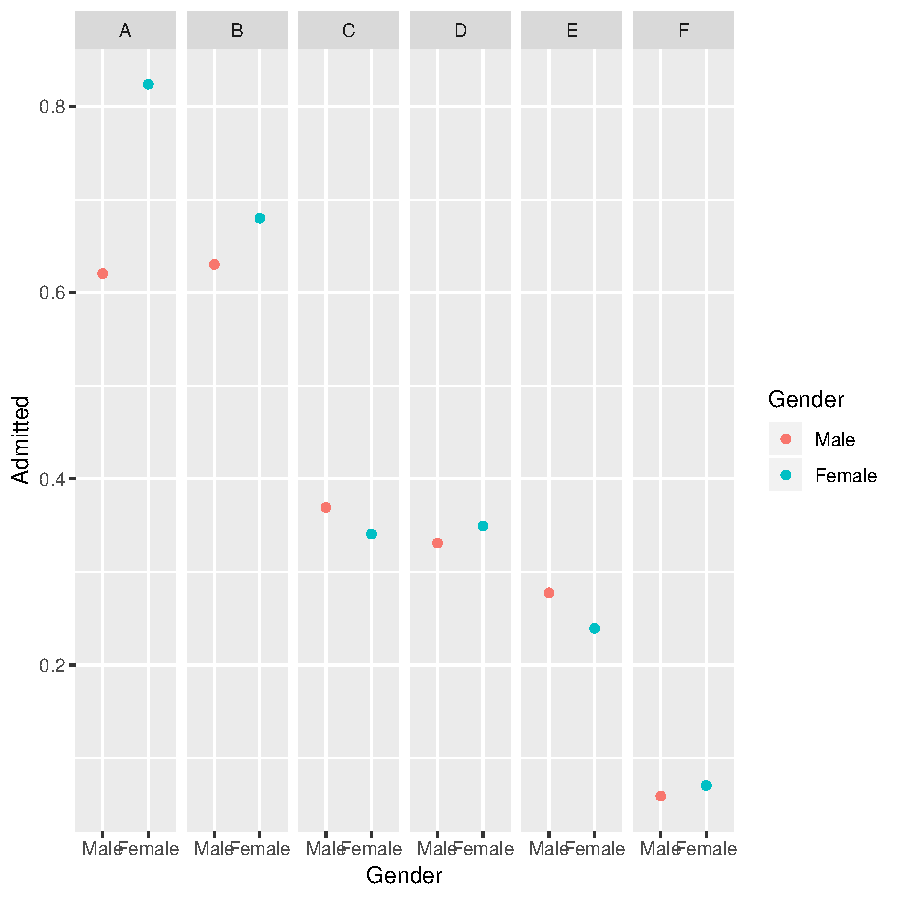
\includegraphics{lect_main-032}

\begin{Schunk}
\begin{Sinput}
> ggplot(data = departmentwise) +
+   geom_point(aes(x = Dept, y = Admitted, colour = Gender)) +
+   facet_grid(~ Gender)
> # or
> 
> qplot(Dept, Admitted, data = departmentwise, colour = Gender) +
+   facet_grid(~ Gender)
\end{Sinput}
\end{Schunk}
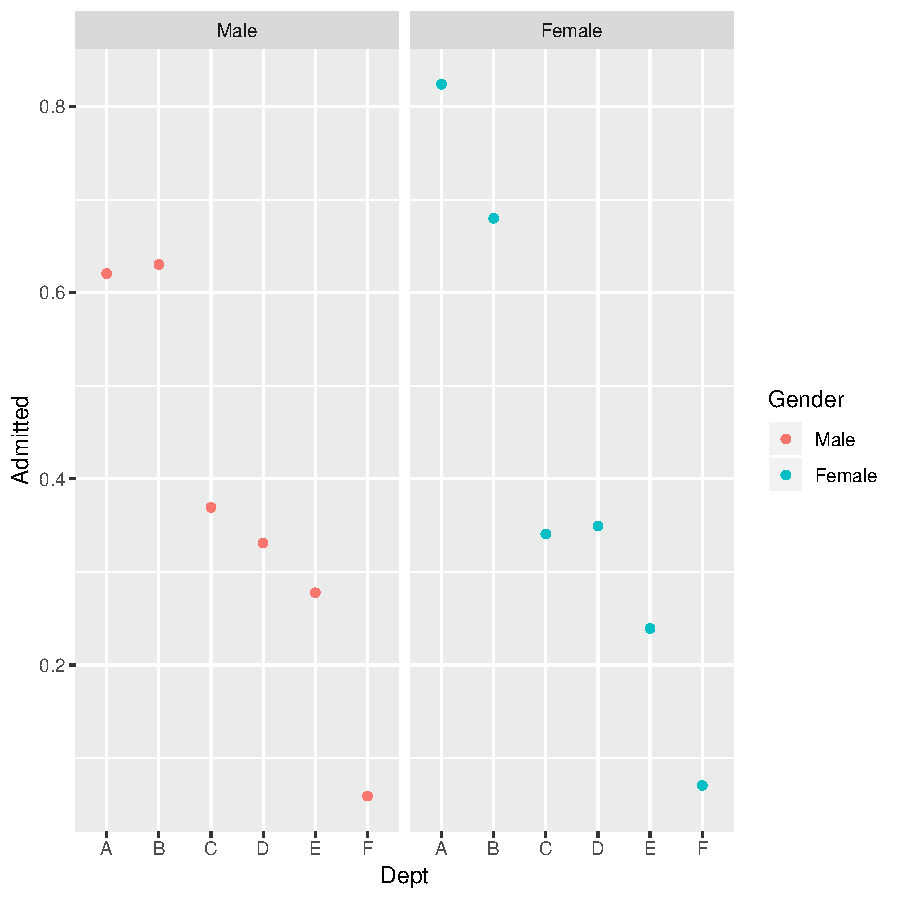
\includegraphics{lect_main-033}

\begin{Schunk}
\begin{Sinput}
> ggplot(data = departmentwise) +
+   geom_point(aes(x = Gender, y = Admitted, colour = Gender)) +
+   facet_grid(Dept ~ Gender)
> # or
> 
> qplot(Gender, Admitted, data = departmentwise, colour = Gender) +
+   facet_grid(Dept ~ Gender)
\end{Sinput}
\end{Schunk}
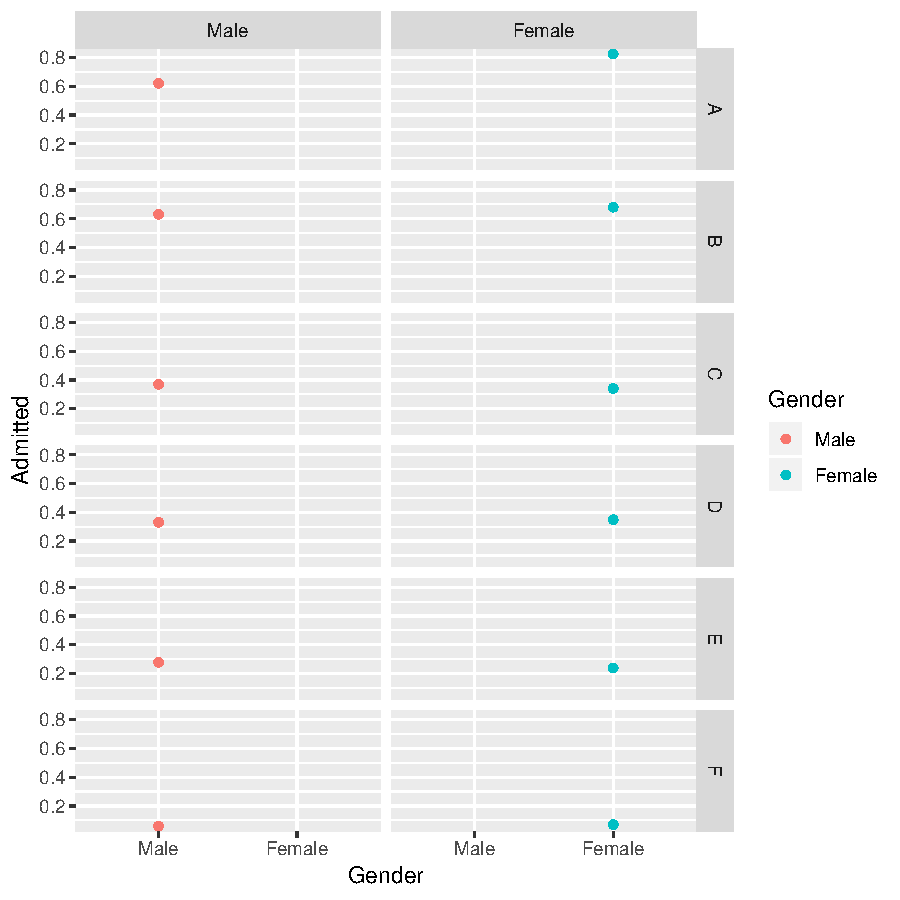
\includegraphics{lect_main-034}

\begin{Schunk}
\begin{Sinput}
> qplot(Gender, Admitted, data = departmentwise, colour = Gender) +
+   facet_grid(Gender ~ Dept)
\end{Sinput}
\end{Schunk}
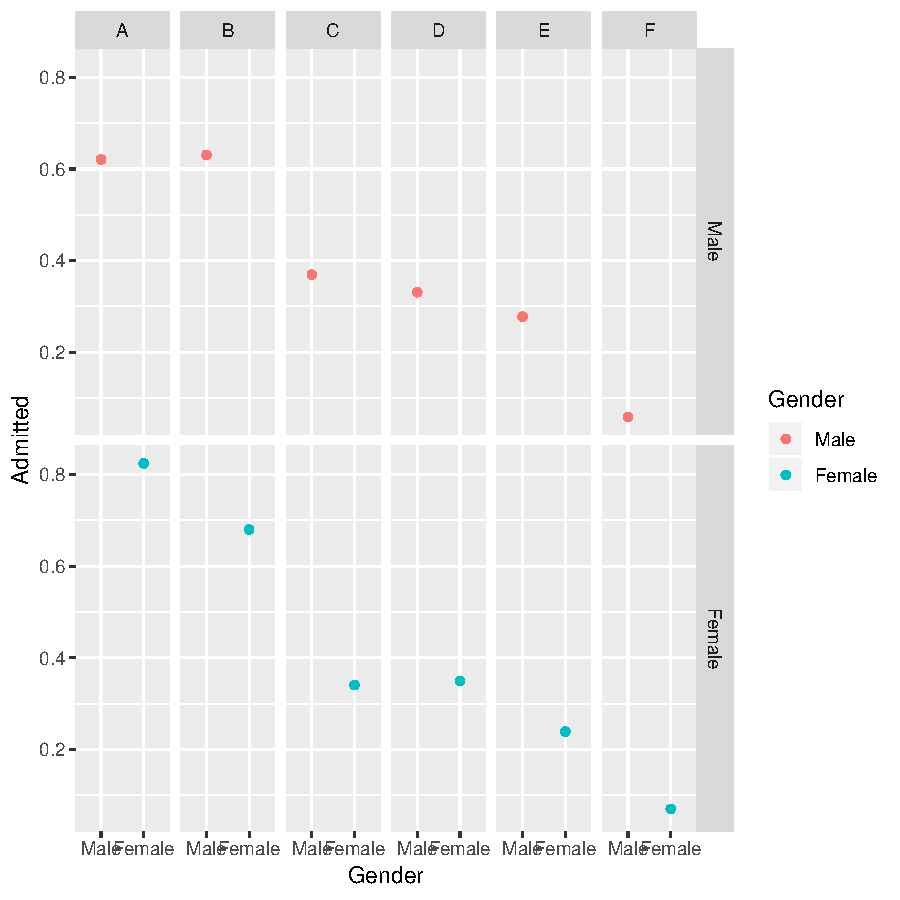
\includegraphics{lect_main-035}

\begin{Schunk}
\begin{Sinput}
> qplot("", Admitted, data = departmentwise, colour = Gender) +
+   facet_grid(~ Gender + Dept)
\end{Sinput}
\end{Schunk}
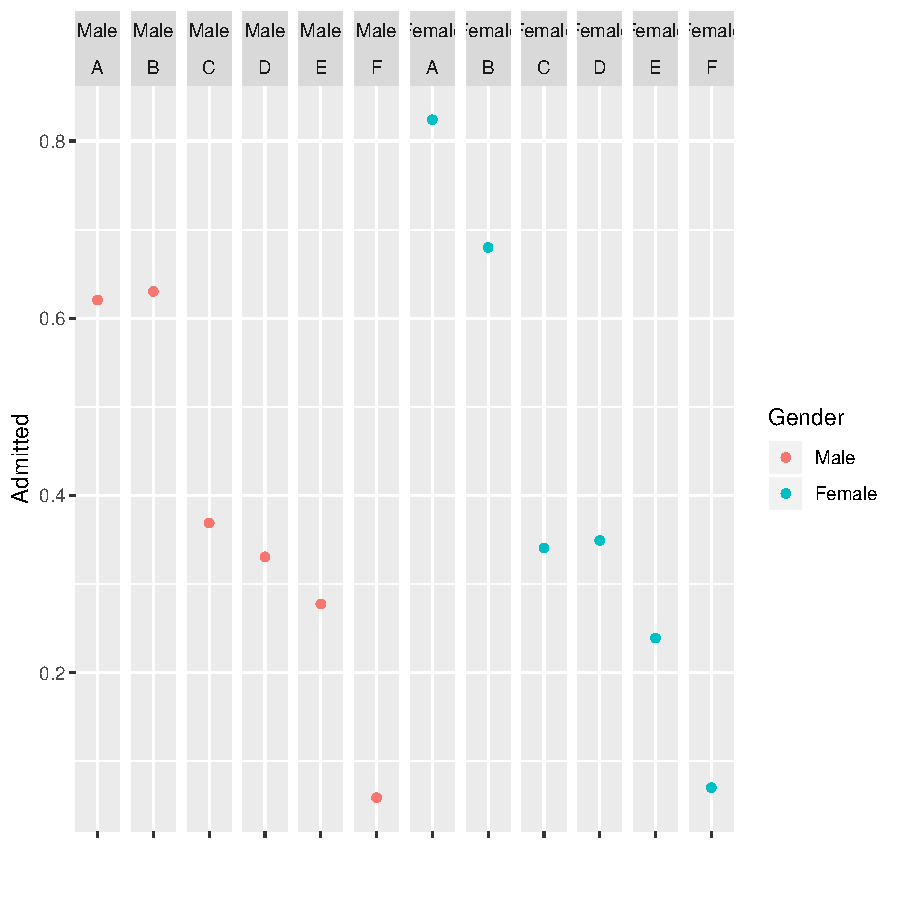
\includegraphics{lect_main-036}

\begin{Schunk}
\begin{Sinput}
> qplot("", Admitted, data = departmentwise, colour = Gender) +
+   facet_grid(~ Dept + Gender)
\end{Sinput}
\end{Schunk}
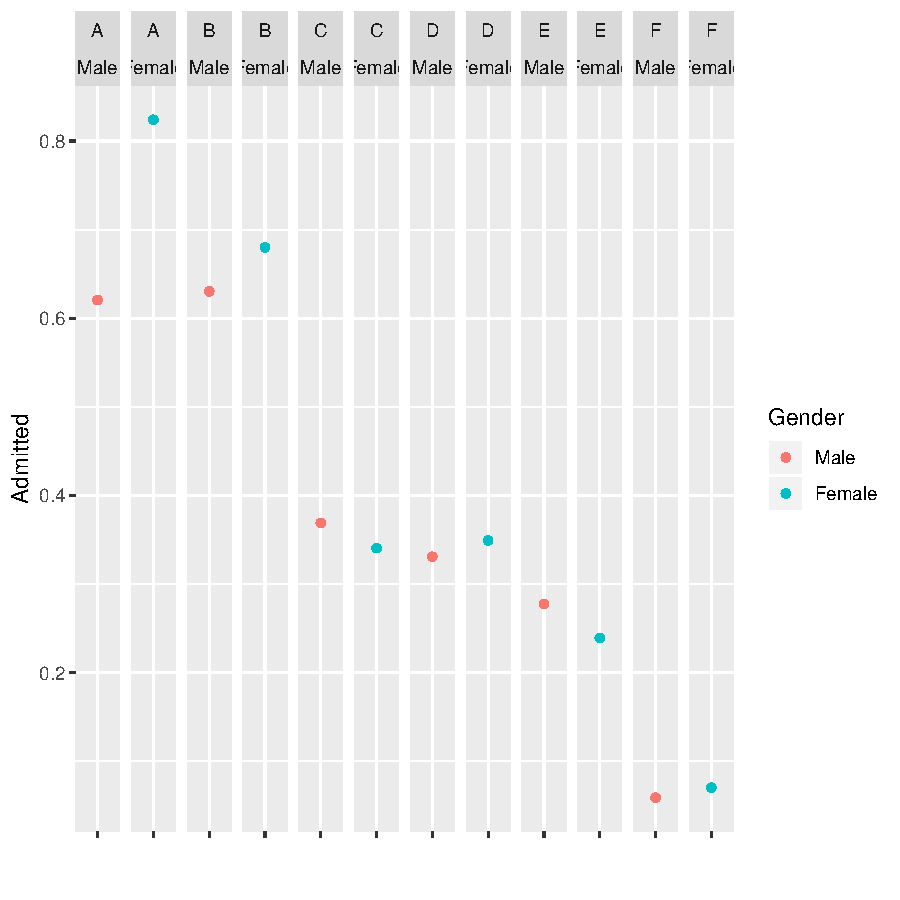
\includegraphics{lect_main-037}


\underline{Note:} \\
We will revisit dot plots in future chapters in Statistical Visualization I \& II.
If you are interested in more sophisticated ones at this time, see this blog
from Nina Zumel where she creates several of the graphs from \cite{Cle94}
via ggplot2: \\
\url{http://www.win-vector.com/blog/2013/02/revisiting-clevelands-the-elements-of-graphing-data-in-ggplot2/}


\newpage


\subsubsection{Mosaic Plots}


The R help page for mosaicplot indicates:
\begin{quotation}
``Plots a mosaic on the current graphics device. [$\ldots$] \\
{\it shade} a logical indicating whether to produce extended mosaic plots, 
or a numeric vector of at most 5 distinct positive numbers giving the absolute values 
of the cut points for the residuals. By default, shade is FALSE, and simple mosaics are created. 
Using shade = TRUE cuts absolute values at 2 and 4.''
\end{quotation}


\begin{Schunk}
\begin{Sinput}
> UCBAdM <- margin.table(UCBAdmissions, 1)
> UCBAdM
\end{Sinput}
\begin{Soutput}
Admit
Admitted Rejected 
    1755     2771 
\end{Soutput}
\begin{Sinput}
> mosaicplot(UCBAdM)
\end{Sinput}
\end{Schunk}
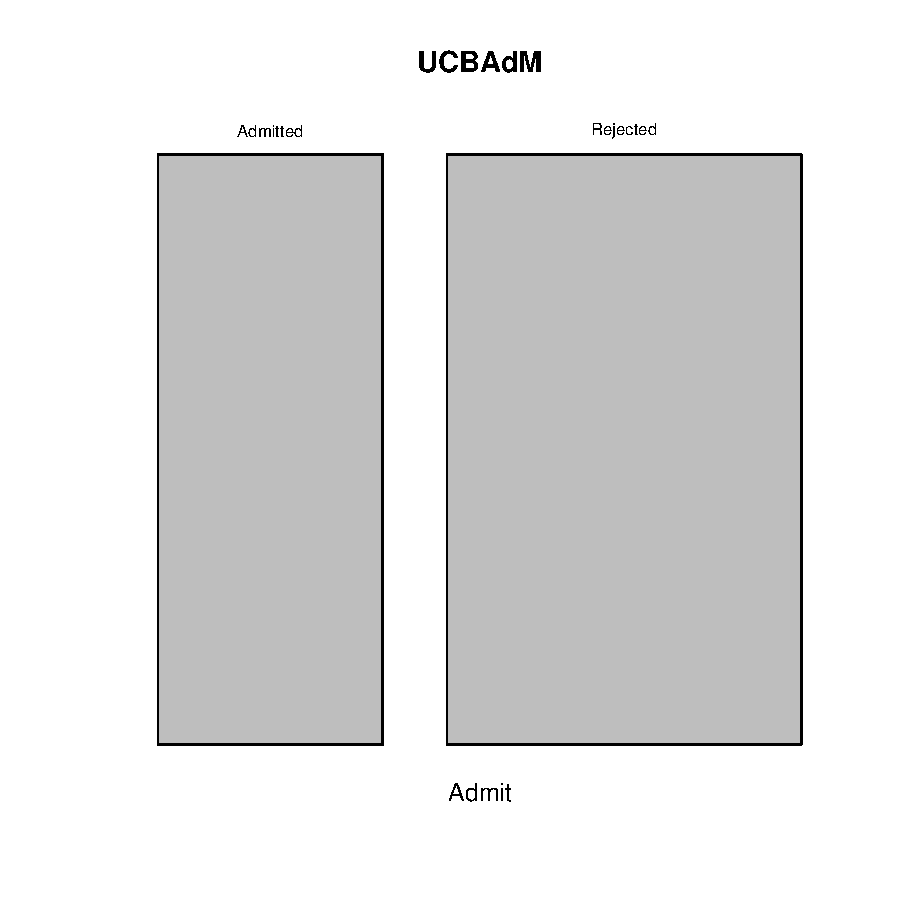
\includegraphics{lect_main-038}

\begin{Schunk}
\begin{Sinput}
> UCBAd <- margin.table(UCBAdmissions, 1:2)
> UCBAd
\end{Sinput}
\begin{Soutput}
          Gender
Admit      Male Female
  Admitted 1198    557
  Rejected 1493   1278
\end{Soutput}
\begin{Sinput}
> mosaicplot(UCBAd)
\end{Sinput}
\end{Schunk}
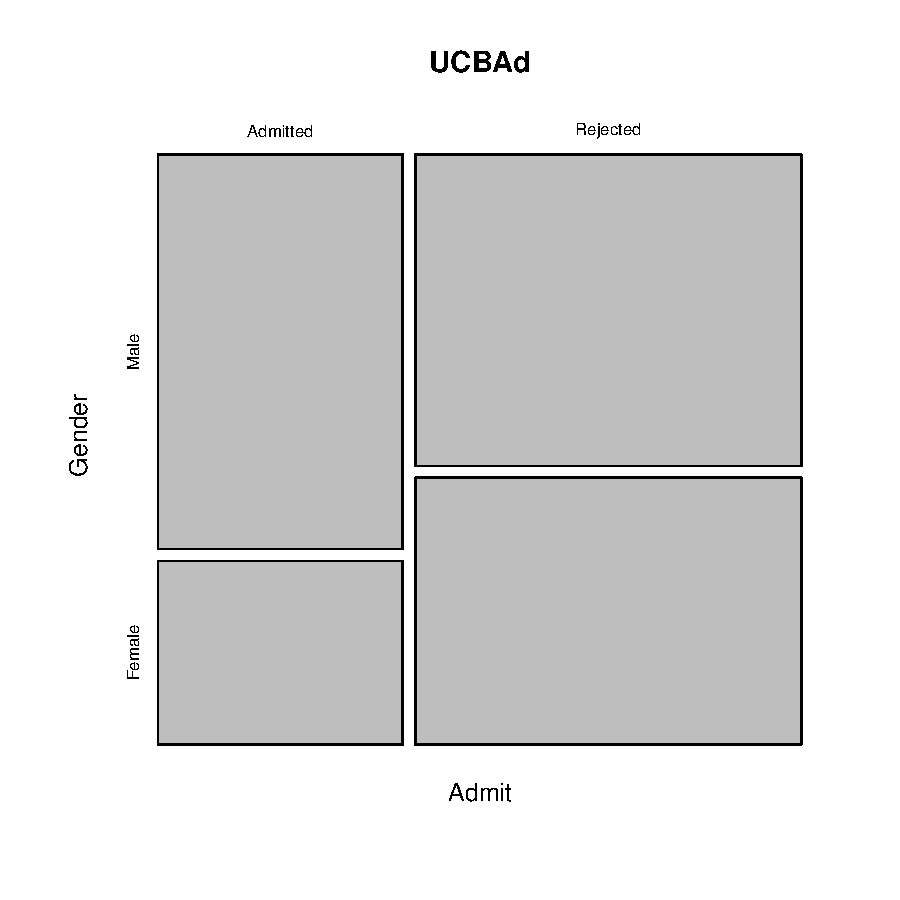
\includegraphics{lect_main-039}

\begin{Schunk}
\begin{Sinput}
> mosaicplot(UCBAdmissions)
\end{Sinput}
\end{Schunk}
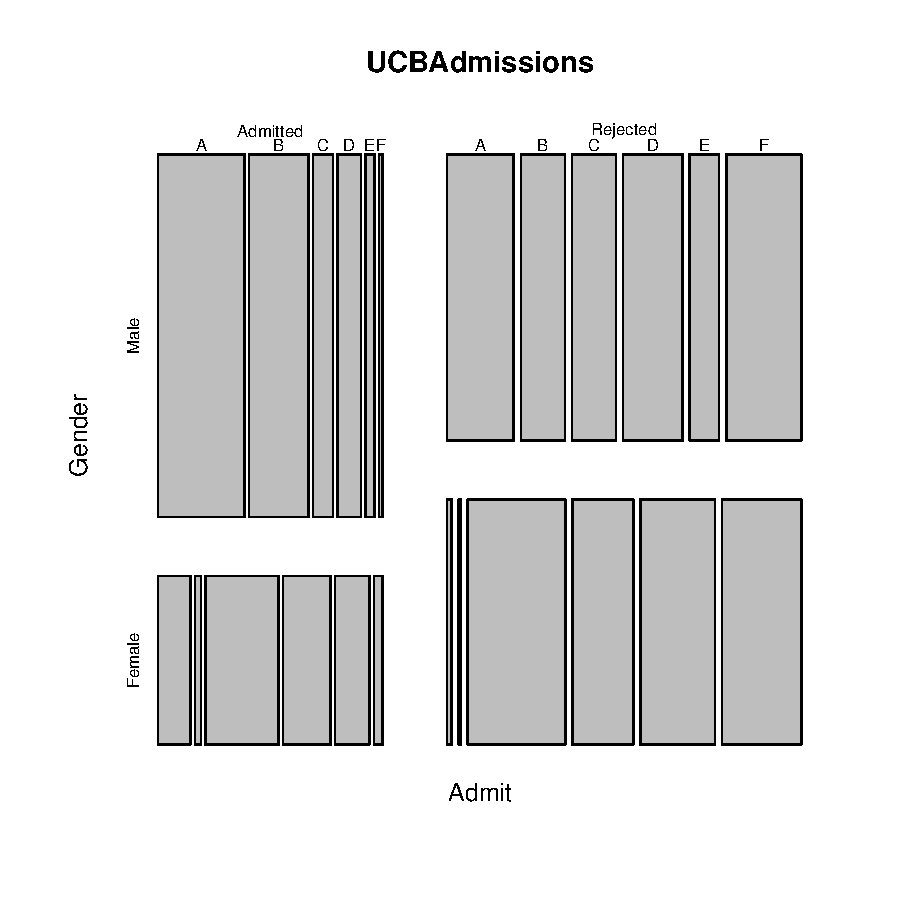
\includegraphics{lect_main-040}


Additional argument {\it shade}: 
\begin{quotation}
``a logical indicating whether to produce extended mosaic plots, or a numeric vector of at most 5 distinct positive numbers giving the absolute values of the cut points for the residuals. By default, shade is FALSE, and simple mosaics are created. Using shade $=$ TRUE cuts absolute values at 2 and 4. \\
Extended mosaic displays visualize standardized residuals of a loglinear model for the table by color and outline of the mosaic's tiles. (Standardized residuals are often referred to a standard normal distribution.) Cells representing negative residuals are drawn in shaded of red and with broken borders; positive ones are drawn in blue with solid borders.''
\end{quotation}

Just using ``shade $=$ TRUE'' assumes an independence model of the variables in the mosaic plot.

\begin{Schunk}
\begin{Sinput}
> mosaicplot(UCBAd, shade = TRUE)
\end{Sinput}
\end{Schunk}
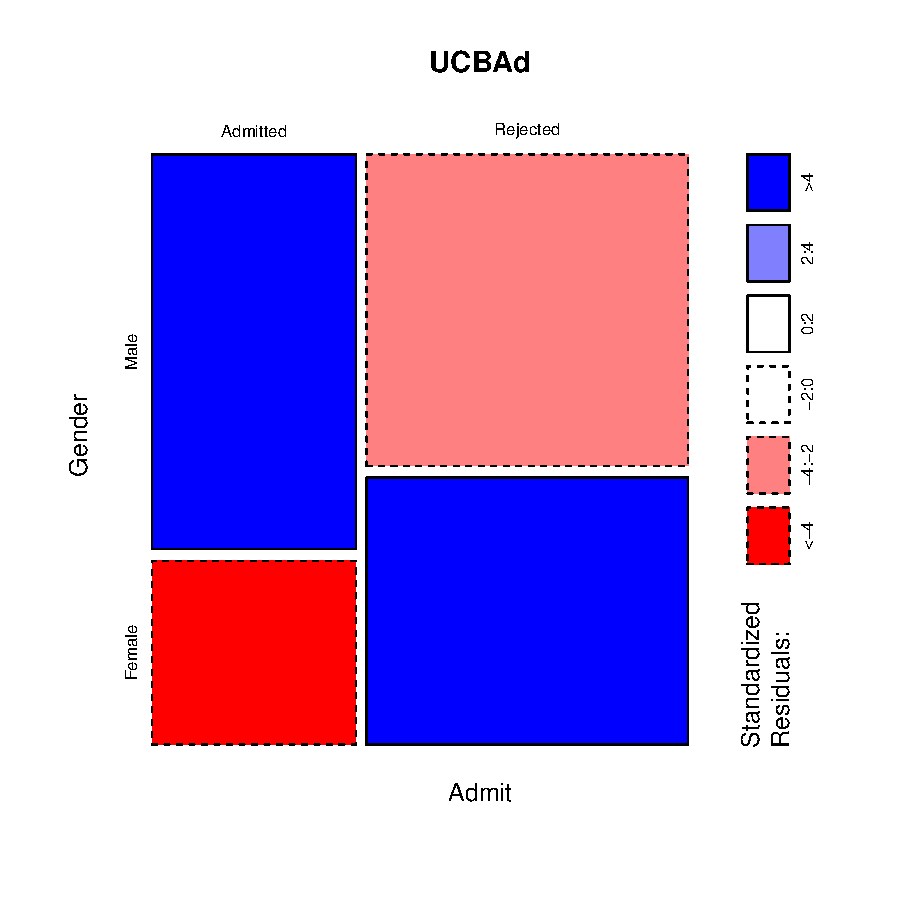
\includegraphics{lect_main-041}

\begin{Schunk}
\begin{Sinput}
> mosaicplot(UCBAdmissions, shade = TRUE)
\end{Sinput}
\end{Schunk}
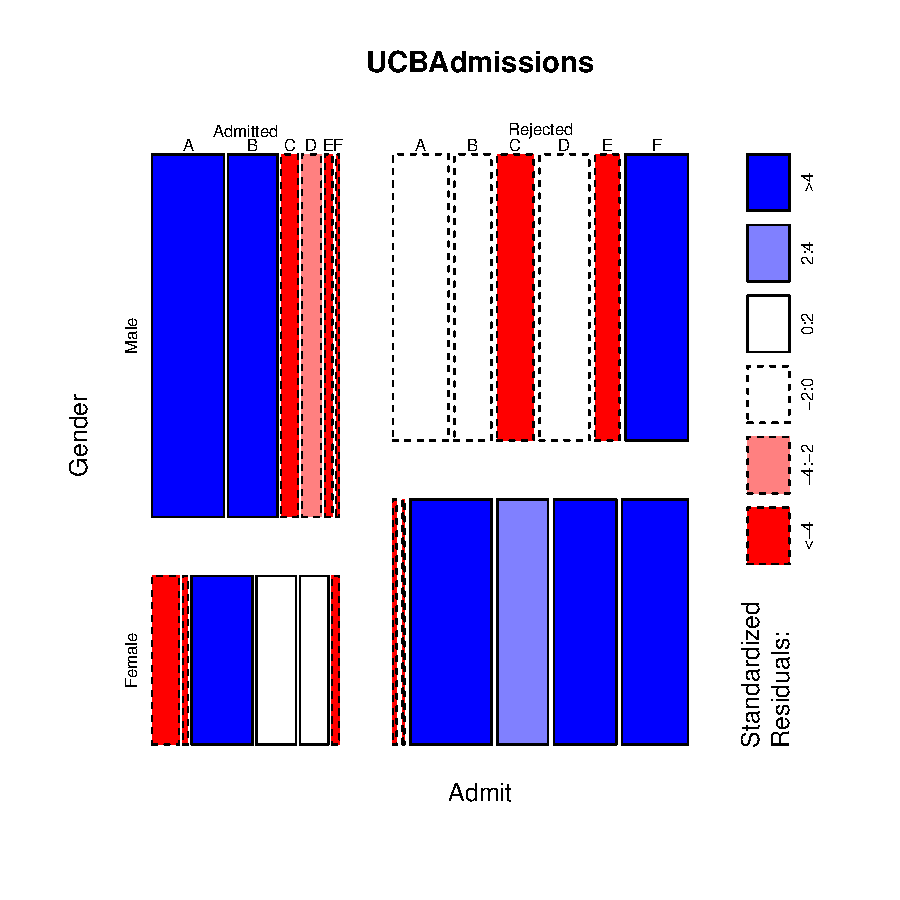
\includegraphics{lect_main-042}

\begin{Schunk}
\begin{Sinput}
> mosaicplot(aperm(UCBAdmissions, 3:1), shade = TRUE)
\end{Sinput}
\end{Schunk}
\includegraphics{lect_main-043}

\begin{Schunk}
\begin{Sinput}
> mosaicplot(aperm(UCBAdmissions, c(2, 3, 1)), shade = TRUE)
\end{Sinput}
\end{Schunk}
\includegraphics{lect_main-044}


Mosaic plots in ggplot2 are produced via the {\it ggmosaic} package.
See \url{https://cran.r-project.org/web/packages/ggmosaic/vignettes/ggmosaic.html}
for further details:


\begin{Schunk}
\begin{Sinput}
> library(ggmosaic)
> library(tibble)
> # function countsToCases taken from
> # http://www.cookbook-r.com/Manipulating_data/Converting_between_data_frames_and_contingency_tables/#countstocases-function
> 
> countsToCases <- function(x, countcol = "Freq") {
+     # Get the row indices to pull from x
+     idx <- rep.int(seq_len(nrow(x)), x[[countcol]])
+ 
+     # Drop count column
+     x[[countcol]] <- NULL
+ 
+     # Get the rows from x
+     x[idx, ]
+ }
> UCBAdmissionstib <- as.tibble(countsToCases(as.data.frame(UCBAdmissions)))
> ggplot(data = UCBAdmissionstib) +
+    geom_mosaic(aes(x = product(Dept, Admit, Gender), fill = factor(Admit)), 
+                divider = mosaic("h"), offset = 0.03) +
+   labs(x = "Gender", y = "Admit") +
+   theme(axis.text.x = element_text(angle = -90, hjust = .1))
\end{Sinput}
\end{Schunk}
\includegraphics{lect_main-045}

\begin{Schunk}
\begin{Sinput}
> ggplot(data = UCBAdmissionstib) +
+    geom_mosaic(aes(x = product(Dept, Gender, Admit), fill = factor(Gender)), 
+                divider = mosaic("h"), offset = 0.03) +
+   labs(x = "Dept:Admit", y = "Gender") +
+   theme(axis.text.x = element_text(angle = -90, hjust = .1)) +
+   guides(fill = guide_legend(title = "Gender", reverse = TRUE))
\end{Sinput}
\end{Schunk}
\includegraphics{lect_main-046}


\newpage


%\begin{figure}[ht]
%\centering{\includegraphics[width=5.0in]{Scans//CNN_2012_Election_Mosaic_Plots.jpg}}
%\caption{\label{CNN_2012_Election_Mosaic_Plots}
%Mosaic Plots in the news, obtained from 
%\url{http://www.cnn.com/election/2012/results/main} on Nov.\ 6, 2012.
%}
%\end{figure}


\newpage


\subsubsection{Spine Plots and Spinograms}


The R help page for spineplot indicates:
\begin{quotation}
``Spine plots are a special case of mosaic plots, 
and can be seen as a generalization of stacked (or highlighted) 
bar plots. Analogously, spinograms are an extension of histograms.''
\end{quotation}


\begin{Schunk}
\begin{Sinput}
> #
> # compare the use of this command without () ...
> #
> spineplot(UCBAd)
\end{Sinput}
\end{Schunk}
\includegraphics{lect_main-047}

\begin{Schunk}
\begin{Sinput}
> #
> # ... and with ()
> #
> (spineplot(UCBAd))
\end{Sinput}
\begin{Soutput}
          Gender
Admit      Male Female
  Admitted 1198    557
  Rejected 1493   1278
\end{Soutput}
\end{Schunk}
\includegraphics{lect_main-048}

\begin{Schunk}
\begin{Sinput}
> (spineplot(t(UCBAd)))
\end{Sinput}
\begin{Soutput}
        Admit
Gender   Admitted Rejected
  Male       1198     1493
  Female      557     1278
\end{Soutput}
\end{Schunk}
\includegraphics{lect_main-049}

\begin{Schunk}
\begin{Sinput}
> (spineplot(margin.table(UCBAdmissions, c(3, 2)), main = "Applications at UCB"))
\end{Sinput}
\begin{Soutput}
    Gender
Dept Male Female
   A  825    108
   B  560     25
   C  325    593
   D  417    375
   E  191    393
   F  373    341
\end{Soutput}
\end{Schunk}
\includegraphics{lect_main-050}

\begin{Schunk}
\begin{Sinput}
> (spineplot(margin.table(UCBAdmissions, c(3, 1)), main = "Admissions at UCB")) 
\end{Sinput}
\begin{Soutput}
    Admit
Dept Admitted Rejected
   A      601      332
   B      370      215
   C      322      596
   D      269      523
   E      147      437
   F       46      668
\end{Soutput}
\end{Schunk}
\includegraphics{lect_main-051}


\newpage


\subsection{Categorical Plots in Mondrian}


According to \url{http://www.theusrus.de/Mondrian/}:
\begin{quotation}
``Mondrian is a general purpose statistical data--visualization system. 
It features outstanding visualization techniques for data of almost any kind, 
and has its particular strength compared to other tools when working with 
{\bf Categorical Data, Geographical Data} and {\bf LARGE Data}. 

All plots in Mondrian are fully linked, and offer various interactions 
and queries. Any case selected in a plot in Mondrian is highlighted in all other plots. 

Currently implemented plots comprise {\bf Mosaic Plot, 
Scatterplots and SPLOM, Maps, Barcharts, Histograms, 
Missing Value Plot, Parallel Coordinates/Boxplots} and {\bf Boxplots y by x}. ''
\end{quotation}


Main references for Mondrian are
\cite{Theu2002}, \cite{Theu2003}, and \cite{TU2009}.
\cite{TU2009} has an associated Web page at \\
\url{http://www.interactivegraphics.org}:
\begin{quotation}
``This site is the web resource for the book ``Interactive Graphics for Data Analysis --- 
Principles and Examples''.

There are links to the most important software tools, all datasets used in the book for 
easy download, and a set of slides which may be used together with the book for a lecture.

The R--code used in the book can be found here as well.''
\end{quotation}


\subsubsection{Installation}


Go to \url{http://www.theusrus.de/Mondrian/}, then follow the link to
the download section on this page. Look over the license condition.
If you agree, then download the most recent version of Mondrian
(currently 1.5b as of 8/28/2013) by right mouse--clicking on the operating system
you use. Save {\it Mondrian.exe} into a directory of your choice. You can start Mondrian
directly (without any additional installation) by mouse--clicking on {\it Mondrian.exe}.

As a test data set, work with the {\it Titanic} data available 
under the {\it Mondrian} {\it Titanic} link or directly
from \url{http://www.theusrus.de/Mondrian/Data/Titanic.txt}.
Save these data locally as {\it Titanic.txt}. Then load them into {\it Mondrian}.


\subsubsection{The Titanic Data in Mondrian}


The {\it Mondrian} description at \url{http://www.theusrus.de/Mondrian/} indicates:
\begin{quotation}
\noindent
``{\bf Titanic} \\[0.2cm]
Data set on the 2201 passengers of the Titanic. Pure categorical with data on 
class, gender, age and survival.''
\end{quotation}


The interactive exploration of the {\it Titanic} data via 
{\it Mondrian} has been further discussed in
\cite{TU2009}, Examples D: The Titanic Disaster Revisited, pp.~183--191.


\underline{Task:} \\
Interactively recreate the nine plots from Figure~\ref{Theus_p186_Fig}
using {\it Mondrian}.


%\begin{figure}[ht]
%\centering{\includegraphics[width=3.0in]{Scans//Theus_p186_Fig.jpg}}
%\caption{\label{Theus_p186_Fig}
%\cite{TU2009}, p.~186, Figure.
%}
%\end{figure}


\newpage


\if\jsprivatechfour 1

\underline{Answer:} \\

%\begin{figure}[ht]
%\centering{\includegraphics[width=3.5in]{Scans//Mondrian_Titanic.jpg}}
%\caption{\label{Mondrian_Titanic}
%{\it Mondrian} output related to \cite{TU2009}, p.~186, Figure.
%}
%\end{figure}


These plots were created via the following settings:
\begin{table}[h]
\small
\centering
\begin{tabular}{|l|l|}
\hline
{\bf (1) Survived:} & {\bf (5) Age:} \\
Bar Chart & Bar Chart \\
Yes & \\
\hline
{\bf (2) Class:} & {\bf (6) Sex:} \\
Bar Chart & Bar Chart \\
Sort By: & \\
~~~~ Relative Selected & \\
\hline
{\bf (3) Class:} & {\bf (7) Age} \\
Bar Chart & Bar Chart \\
Spine Plot & Spine Plot \\
\hline
{\bf (4) Sex \& Class:} & {\bf (8) Sex:} \\
Mosaic Plot & Bar Chart \\
 & Spine Plot \\
\hline
 & {\bf (9) Class \& Age \& Sex:} \\
 & Mosaic Plot \\
 & Display As: \\
 & ~~~~ Same Bin Size \\
\hline
\end{tabular}
\end{table}


\else
{\bf Additional details will be provided after class.}
\fi


% Data description from http://rosuda.org/mondrian/
%Here are some sample data sets, which are ready to load and test with 
%Mondrian (make sure to save the link directly to preserve the tabs!):

%Titanic 
%Data set on the 2201 passengers of the Titanic. Pure categorical with data on 
%class, gender, age and survival. 

%Pollen 
%Fake data set with hidden feature, which is easily found with $\alpha$-channel features. 

%Olive Oils 
%Data set on Italian olive oils. Several fatty acids have been measured which 
%allow to separate the different regions from Italy. 

%Berlin (old map format) 
%Election and socio-economic data on the city of Berlin, shortly after the Berlin Wall 
%was torn down. Includes a polygon of the districts of Berlin.

%US Election 2004 (new map format)
%Data on the 2004 US presidential election. Includes polygons of the Counties of the US. 
%Data courtesy of GeoVISTA (http://www.personal.psu.edu/users/a/c/acr181/election.html)


\newpage


\subsubsection{The Titanic Data in iPlots}

{\it iPlots} is an interactive graphics package for R,
further described in \cite{TU2004} and
accessible at
\url{http://cran.r-project.org/web/packages/iplots/index.html}.
{\it iPlots} is closely related to {\it Mondrian}.
In the example below, we will reproduce some of the plots
via {\it iPlots} that were previously created via {\it Mondrian}.

\begin{Schunk}
\begin{Sinput}
> Sys.setenv(JAVA_HOME = "C:/Program Files/Java/jdk-11.0.1/")
> library(iplots)
> TitanicMondrian <- read.table("http://www.theusrus.de/Mondrian/Data/Titanic.txt",
+                               header = TRUE)
> summary(TitanicMondrian)
\end{Sinput}
\begin{Soutput}
    Class        Age           Sex       Survived  
 Crew  :885   Adult:2092   Female: 470   No :1490  
 First :325   Child: 109   Male  :1731   Yes: 711  
 Second:285                                        
 Third :706                                        
\end{Soutput}
\begin{Sinput}
> ibar(TitanicMondrian$Survived)
\end{Sinput}
\begin{Soutput}
ID:1 Name: "Barchart (TitanicMondrian$Survived)"
\end{Soutput}
\begin{Sinput}
> iplot.rotate(1)
> iset.select(TitanicMondrian$Survived == "Yes")
> ibar(TitanicMondrian$Class)
\end{Sinput}
\begin{Soutput}
ID:2 Name: "Barchart (TitanicMondrian$Class)"
\end{Soutput}
\begin{Sinput}
> iplot.rotate(1)
> ibar(TitanicMondrian$Class, isSpine = TRUE)
\end{Sinput}
\begin{Soutput}
ID:3 Name: "Barchart (TitanicMondrian$Class)"
\end{Soutput}
\begin{Sinput}
> iplot.rotate(1)
> ibar(TitanicMondrian$Age)
\end{Sinput}
\begin{Soutput}
ID:4 Name: "Barchart (TitanicMondrian$Age)"
\end{Soutput}
\begin{Sinput}
> iplot.rotate(1)
> imosaic(TitanicMondrian$Sex, TitanicMondrian$Class)
\end{Sinput}
\begin{Soutput}
ID:5 Name: "Mosaic plot (TitanicMondrian$Sex, TitanicMondrian$Class)"
\end{Soutput}
\begin{Sinput}
> imosaic(TitanicMondrian$Sex, TitanicMondrian$Class, TitanicMondrian$Age)
\end{Sinput}
\begin{Soutput}
ID:6 Name: "Mosaic plot (TitanicMondrian$Sex, TitanicMondrian$Class, TitanicMondrian$Age)"
\end{Soutput}
\begin{Sinput}
> iset.selectNone()
> iobj.list()
\end{Sinput}
\begin{Soutput}
[[1]]
PlotText(labels=2,coord=0/0,visible=true) 

[[2]]
PlotText(labels=4,coord=0/0,visible=true) 
\end{Soutput}
\begin{Sinput}
> for (i in 1:length(iobj.list())) 
+   iobj.rm() # remove all objects
> iplot.list()
\end{Sinput}
\begin{Soutput}
[[1]]
ID:1 Name: "Barchart (TitanicMondrian$Survived)"

[[2]]
ID:2 Name: "Barchart (TitanicMondrian$Class)"

[[3]]
ID:3 Name: "Barchart (TitanicMondrian$Class)"

[[4]]
ID:4 Name: "Barchart (TitanicMondrian$Age)"

[[5]]
ID:5 Name: "Mosaic plot (TitanicMondrian$Sex, TitanicMondrian$Class)"

[[6]]
ID:6 Name: "Mosaic plot (TitanicMondrian$Sex, TitanicMondrian$Class, TitanicMondrian$Age)"
\end{Soutput}
\begin{Sinput}
> for (i in 1:length(iplot.list()))
+   iplot.off() # close all windows
> 
> 
> #iset.rm() # remove this iset
\end{Sinput}
\end{Schunk}


\newpage


\subsection{Further Reading}

Additional sources for the visualization of categorical data are:

\begin{itemize}
\item \cite{BG98}

\item \cite{Fr2000VCD}

\item \cite{Hof2007}

\item \cite{TU2009}

\end{itemize}


~\\[0.5in]

%\begin{figure}[ht]
%\centering{\includegraphics[height=4in]{Scans//Cartoonstock_Pizza.png}}
%\caption{\label{Cartoonstock_Pizza}
%\url{http://www.cartoonstock.com/cartoonview.asp?start=7&search=main&catref=rde1808&MA_Artist=&MA_Category=&ANDkeyword=statistics&ORkeyword=&TITLEkeyword=&NEGATIVEkeyword=}, 
%Cartoon.
%}
%\end{figure}


\newpage


~\\[2cm]


%\begin{figure}[ht]
%\centering{\includegraphics[height=4in]{Scans//BarChartsTaller.jpg}}
%\caption{\label{BarChartsTaller}
%\url{http://www.dxbydt.com/bars-pies-using-ggplot2/},
%Cartoon.
%}
%\end{figure}


\newpage


%\SweaveInput{lect_chapter5.Rnw}
%\SweaveInput{lect_chapter6.Rnw}
%\SweaveInput{lect_chapter1.Rnw}
%
%\SweaveInput{lect_chapter2.Rnw}
%\SweaveInput{lect_chapter3.Rnw}
%\SweaveInput{lect_chapter9.Rnw}
%\SweaveInput{lect_chapter7.Rnw}
%\SweaveInput{lect_chapter8.Rnw}
%\SweaveInput{lect_chapter10.Rnw}


\setcounter{page}{1}
\addcontentsline{toc}{section}{References}

\bibliography{references}


\vspace*{1cm}

\centering{\bf \LARGE --- THE END ---}~\\[1cm]

%\begin{figure}[ht]
%\centering{\includegraphics[height=3in]{Scans//Cartoonstock_FallingArrow.jpg}}
%\caption{\label{Cartoonstock_FallingArrow}
%\url{http://www.cartoonstock.com/blowup_stock.asp?imageref=vsh0184&artist=Shirvanian,+Vahan&topic=statistics+}, 
%Cartoon.
%}
%\end{figure}


\end{document}

